% =============================================================================
% Parte 2 — PX4 + ROS 2 con px4_examples, paso a paso
% Vespo UAV
%
% Para presentar después de la Parte 1 (parte1.tex). Lo técnico a detalle
% (cada mensaje campo por campo, el código completo) está en referencia.tex.
%
% Compilar:  latexmk -pdf main.tex
% =============================================================================
\documentclass[aspectratio=169,10pt]{beamer}
% =============================================================================
% PX4 + ROS 2 con px4_examples — Vespo UAV
%
% Compilar:  latexmk -pdf main.tex      (o pdflatex dos veces, por los índices)
% Necesita:  texlive-latex-extra texlive-lang-spanish texlive-pictures
%            texlive-fonts-recommended
%
% Cada sección vive en secciones/NN_nombre.tex. Todo lo que se cita del código
% sale de src/px4_examples/src/*.cpp.
% =============================================================================
% (el \documentclass va en cada presentación)

\usepackage[utf8]{inputenc}
\usepackage[T1]{fontenc}
\usepackage[spanish,es-nodecimaldot,es-noshorthands]{babel}
\usepackage{amsmath,amssymb}
\usepackage{booktabs}
\usepackage{graphicx}
\usepackage{xcolor}
\usepackage{listings}
\usepackage[most]{tcolorbox}
\usepackage{tikz}
\usetikzlibrary{arrows.meta,positioning,shapes.geometric,shapes.misc,calc,fit,backgrounds,decorations.pathreplacing}
\usepackage{multicol}
\usepackage{pifont}
% Lo que imprime vespo en la terminal
\DeclareUnicodeCharacter{2714}{\ding{51}}
\DeclareUnicodeCharacter{2718}{\ding{55}}
\DeclareUnicodeCharacter{2500}{\textendash}

\graphicspath{{img/}{img/px4docs/}{img/render/}{../../../x500_retos/docs/img/}}

% --- Tema: el de la intro a ROS2 ---------------------------------------------
\usetheme{default}
\useoutertheme{infolines}
\setbeamertemplate{headline}{}
\setbeamercolor{author in head/foot}{fg=black,bg=white}
\setbeamercolor{title in head/foot}{fg=blue!70!black,bg=white}
\setbeamercolor{date in head/foot}{fg=black,bg=white}
\setbeamercolor{section in toc}{fg=blue!70!black}
\setbeamertemplate{section in toc}[circle]
\setbeamercolor{frametitle}{fg=black,bg=white}
\setbeamerfont{frametitle}{size=\Large}
\setbeamertemplate{frametitle}{%
  \vskip0.4em
  \begin{beamercolorbox}[wd=\paperwidth,leftskip=0.3em,rightskip=0.3em]{frametitle}%
    \usebeamerfont{frametitle}\insertframetitle\hfill
    \raisebox{-0.45em}{
\includegraphics[height=1.6em]{vespo_logo}}%
  \end{beamercolorbox}}
\setbeamertemplate{caption}[numbered]
\setbeamertemplate{itemize items}[circle]
\setbeamercolor{itemize item}{fg=blue!70!black}
\setbeamercolor{enumerate item}{fg=blue!70!black}

% --- Colores y cajas -------------------------------------------------------------
\definecolor{azul}{RGB}{40,80,180}
\definecolor{azulclaro}{RGB}{232,238,252}
\definecolor{verde}{RGB}{0,128,0}
\definecolor{verdeclaro}{RGB}{236,250,236}
\definecolor{rojo}{RGB}{190,30,30}
\definecolor{naranja}{RGB}{230,120,10}
\definecolor{gris}{RGB}{110,110,110}

% Idea clave: caja azul redondeada con sombra.
\newtcolorbox{idea}[1][]{enhanced,colback=azulclaro,colframe=azul!40,arc=2mm,
  boxrule=0.4pt,drop shadow,left=1.5mm,right=1.5mm,top=1mm,bottom=1mm,#1}
% Ojo: lo que suele salir mal.
\newtcolorbox{ojo}[1][]{enhanced,colback=red!5,colframe=rojo!60,arc=2mm,boxrule=0.4pt,
  drop shadow,left=1.5mm,right=1.5mm,top=1mm,bottom=1mm,
  title={\small\bfseries Ojo},fonttitle=\small,coltitle=white,colbacktitle=rojo!80,#1}
% Salida de terminal: barra verde con el comando.
\newtcolorbox{terminal}[1]{enhanced,colback=verdeclaro,colframe=verde,arc=1mm,boxrule=0.6pt,
  title={\ttfamily\small #1},fonttitle=\ttfamily\small,coltitle=white,colbacktitle=verde,
  left=1mm,right=1mm,top=0.5mm,bottom=0.5mm,fontupper=\ttfamily\scriptsize}

% --- Código ----------------------------------------------------------------------
\renewcommand{\lstlistingname}{Código}
\lstset{
  basicstyle=\ttfamily\scriptsize,
  keywordstyle=\color{azul}\bfseries,
  commentstyle=\color{gris}\itshape,
  stringstyle=\color{verde},
  frame=single, rulecolor=\color{black},
  breaklines=true, columns=fullflexible, keepspaces=true,
  showstringspaces=false, captionpos=b, tabsize=2,
  xleftmargin=2pt, xrightmargin=2pt, aboveskip=4pt, belowskip=2pt,
  literate=
    {á}{{\'a}}1 {é}{{\'e}}1 {í}{{\'i}}1 {ó}{{\'o}}1 {ú}{{\'u}}1
    {Á}{{\'A}}1 {É}{{\'E}}1 {Í}{{\'I}}1 {Ó}{{\'O}}1 {Ú}{{\'U}}1
    {ñ}{{\~n}}1 {Ñ}{{\~N}}1 {ü}{{\"u}}1 {¿}{{?`}}1 {¡}{{!`}}1
    {°}{{$^\circ$}}1 {²}{{$^2$}}1 {·}{{$\cdot$}}1
    {→}{{$\rightarrow$}}2 {←}{{$\leftarrow$}}2 {≈}{{$\approx$}}1
    {▲}{{$\blacktriangle$}}1 {►}{{$\blacktriangleright$}}1 {│}{{|}}1 {─}{{-}}1
    {┌}{{+}}1 {┐}{{+}}1 {└}{{+}}1 {┘}{{+}}1 {├}{{+}}1 {┤}{{+}}1 {┼}{{+}}1
}
\lstdefinestyle{cpp}{language=C++,morekeywords={override,nullptr,constexpr,auto}}
\lstdefinestyle{bash}{language=bash,morekeywords={ros2,vespo,colcon}}
\lstdefinelanguage{yaml}{morecomment=[l]\#,morestring=[b]"}

% --- Atajos ---------------------------------------------------------------------
\newcommand{\cmd}[1]{\texttt{#1}}
\newcommand{\ok}{{\color{verde}\checkmark}}
\newcommand{\mal}{{\color{rojo}$\times$}}

% Al empezar cada sección: el contenido con la sección actual resaltada.
\AtBeginSection[]{%
  \begin{frame}{Contenido}
    \begin{multicols}{2}\scriptsize
      \tableofcontents[currentsection]
    \end{multicols}
  \end{frame}}

% Láminas que se arman paso a paso: en TikZ, "visible on=<3->" muestra un
% nodo desde el paso 3 y "alt=<2>{fill=...}{fill=...}" lo resalta en el paso 2.
\tikzset{
  invisible/.style={opacity=0,text opacity=0},
  visible on/.style={alt={#1{}{invisible}}},
  alt/.code args={<#1>#2#3}{\alt<#1>{\pgfkeysalso{#2}}{\pgfkeysalso{#3}}},
}
\newcommand{\credito}[1]{{\tiny\color{gris}#1}}

% El x500 recortado (tools/renders_x500.py + tools/recortar_iconos.py).
% \dronarriba{ancho}: visto desde arriba, la nariz hacia arriba de la imagen.
% Para girarlo a un yaw (0 = norte, positivo hacia el este) en TikZ: \node[rotate=-yaw].
\newcommand{\dronarriba}[1]{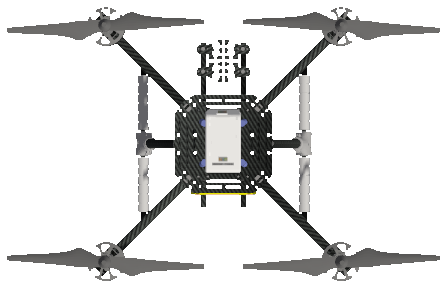
\includegraphics[width=#1]{x500_icono}}
\newcommand{\dronlado}[1]{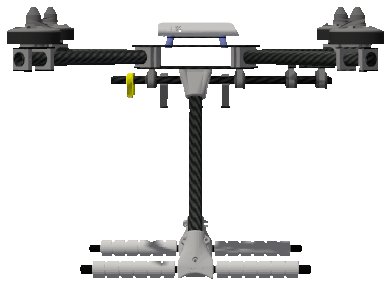
\includegraphics[width=#1]{x500_lado_icono}}


\title[PX4 + ROS 2 paso a paso]{PX4 + ROS 2 con px4\_examples}
\subtitle{Paso a paso: de instalar a volar el x500 con tu propio nodo (Parte 2)}
\author[Imad Cabrera]{Imad Jared Cabrera Trejo}
\institute[Vespo UAV]{Vespo UAV Drones Autónomos}
\date{11 de noviembre de 2026}

\begin{document}

\begin{frame}[plain]
  \begin{tikzpicture}[remember picture,overlay]
    \node at (current page.center) {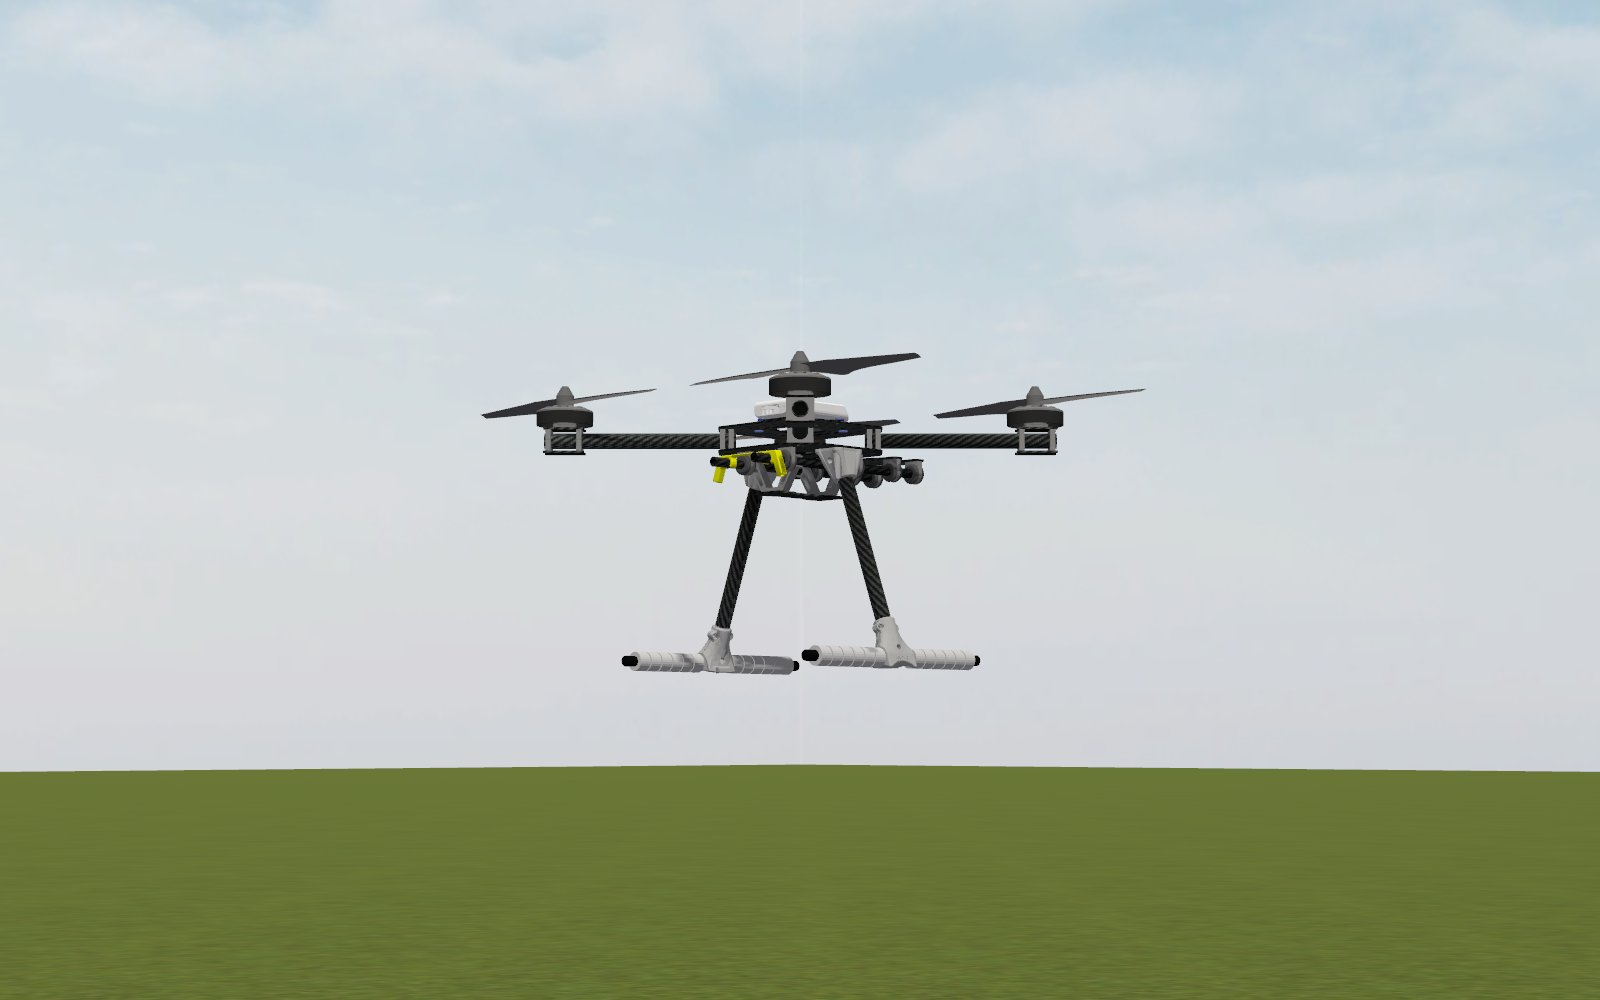
\includegraphics[width=\paperwidth]{x500_volando}};
    \fill[white,opacity=0.8] ([yshift=-1.5cm]current page.north west) rectangle ([yshift=-4.5cm]current page.north east);
    \node[font=\LARGE\bfseries] at ([yshift=-2.4cm]current page.north) {PX4 + ROS 2 con px4\_examples};
    \node[font=\normalsize] at ([yshift=-3.2cm]current page.north) {Paso a paso: de instalar a volar el x500 con tu propio nodo (Parte 2)};
    \node[font=\scriptsize] at ([yshift=-3.9cm]current page.north) {Imad Jared Cabrera Trejo · Vespo UAV · 11 de noviembre de 2026};
    \node[anchor=south east] at ([xshift=-0.3cm,yshift=0.3cm]current page.south east) {
\includegraphics[height=1.1cm]{vespo_logo}};
  \end{tikzpicture}
\end{frame}

\begin{frame}{Hoy}
  \begin{columns}[c]
    \column{0.55\textwidth}
    \begin{enumerate}\small
      \item \textbf{Instalar} todo con \cmd{vespo}, desde cero.
      \item \textbf{Repaso} del x500 y de PX4 en 4 láminas.
      \item Cómo \textbf{habla} ROS 2 con PX4.
      \item \cmd{shared\_ptr}: lo único de C++ que hoy hace falta.
      \item \textbf{Escuchar} al dron.
      \item \textbf{Volar en offboard}: \cmd{square\_mission} cuadro por cuadro.
      \item \textbf{Volar con comandos}: \cmd{goto\_mission} y \cmd{return\_home}.
      \item \textbf{Tu primer reto}: la estrella del show.
      \item \textbf{Cuando algo no jala}.
    \end{enumerate}
    \column{0.42\textwidth}\centering
    \dronarriba{0.8\linewidth}
  \end{columns}
\end{frame}

% =============================================================================
\section{Instalar todo con vespo}
% =============================================================================

% La barra de pasos de arriba de cada lámina de esta sección: \camino{n} resalta el paso n.
\newcommand{\camino}[1]{%
  \begin{tikzpicture}[every node/.style={font=\tiny}]
    \foreach \i/\t in {1/clonar,2/bootstrap,3/init,4/doctor,5/build,6/up,7/ejemplo,8/down} {
      \ifnum\i<#1 \def\cc{verde}\def\ff{verde!20}\else\ifnum\i=#1 \def\cc{azul}\def\ff{yellow!50}\else\def\cc{gray!60}\def\ff{white}\fi\fi
      \node[circle,draw=\cc,fill=\ff,line width=0.8pt,minimum size=0.42cm,font=\tiny\bfseries] (c\i) at (\i*1.62,0) {\i};
      \node[below=0.02cm of c\i,text=\cc] {\t};
      \ifnum\i>1 \pgfmathtruncatemacro{\p}{\i-1}\draw[gray!60] (c\p) -- (c\i);\fi
    }
  \end{tikzpicture}\par\vspace{0.2em}}

\begin{frame}{El camino completo}
  \centering
  \begin{tikzpicture}[every node/.style={font=\scriptsize,align=center},
      st/.style={draw=azul,fill=azulclaro,rounded corners,minimum width=2.6cm,minimum height=1.25cm,text width=2.5cm}]
    \node[st] (a) at (0,1.6) {\textbf{1 Clonar}\\\cmd{git clone}\\una sola vez};
    \node[st] (b) at (3.4,1.6) {\textbf{2 bootstrap}\\instala ROS 2\\y \cmd{vespo}};
    \node[st] (c) at (6.8,1.6) {\textbf{3 vespo init}\\PX4, Gazebo, QGC\\y compila};
    \node[st] (d) at (10.2,1.6) {\textbf{4 vespo doctor}\\¿todo en orden?};
    \node[st,fill=yellow!25] (e) at (10.2,-0.6) {\textbf{5 vespo build}\\cuando cambias\\código};
    \node[st,fill=yellow!25] (f) at (6.8,-0.6) {\textbf{6 vespo up -{}-sim}\\levanta la\\simulación};
    \node[st,fill=yellow!25] (g) at (3.4,-0.6) {\textbf{7 ros2 run}\\corre un\\ejemplo};
    \node[st,fill=yellow!25] (h) at (0,-0.6) {\textbf{8 vespo down}\\apaga todo};
    \draw[-{Stealth},thick] (a) -- (b); \draw[-{Stealth},thick] (b) -- (c); \draw[-{Stealth},thick] (c) -- (d);
    \draw[-{Stealth},thick] (d) -- (e); \draw[-{Stealth},thick] (e) -- (f); \draw[-{Stealth},thick] (f) -- (g);
    \draw[-{Stealth},thick] (g) -- (h);
    \draw[decorate,decoration={brace,amplitude=5pt,mirror},gris] (-1.3,0.5) -- (-1.3,2.7)
      node[midway,left=6pt,font=\tiny,text=gris] {una vez};
    \draw[decorate,decoration={brace,amplitude=5pt},gris] (11.5,0.0) -- (11.5,-1.2)
      node[midway,right=6pt,font=\tiny,text=gris,text width=1.3cm] {cada día};
  \end{tikzpicture}
  \vspace{0.5em}

  \raggedright\small Los pasos \textbf{1 a 4} se hacen una vez por computadora. Del \textbf{5 al 8} es lo de
  todos los días.
\end{frame}

\begin{frame}{Antes de empezar}
  \camino{0}
  \begin{columns}[t]
    \column{0.48\textwidth}
    \begin{idea}[title={\small\bfseries Lo que necesitas},coltitle=black,colbacktitle=azulclaro]
      \small
      \begin{itemize}
        \item \textbf{Ubuntu 24.04} (no otra versión: es la única con ROS 2 Jazzy).
        \item \textbf{\textasciitilde30 GB libres}: PX4 y Gazebo solos ocupan \textasciitilde15 GB.
        \item \textbf{Buen internet}: la primera vez baja varios GB.
        \item Tu \textbf{contraseña} (pide \cmd{sudo} para instalar).
        \item \textbf{1 a 2 horas} la primera vez.
      \end{itemize}
    \end{idea}
    \column{0.48\textwidth}
    \begin{ojo}[title={\small\bfseries Conecta el cargador}]
      \small La simulación usa mucho CPU y tarjeta de video. Con batería la laptop se pone lenta y puede
      \textbf{apagarse sola} a media simulación.
    \end{ojo}
    \begin{idea}
      \small Si algo se corta (internet, batería), \textbf{no pasa nada}: vuelves a correr el mismo comando y
      sigue donde iba.
    \end{idea}
  \end{columns}
\end{frame}

\begin{frame}[fragile]{Paso 1: clonar el repositorio}
  \camino{1}
  \begin{lstlisting}[style=bash]
sudo apt install git                                   # si no lo tienes
cd ~                                                   # en tu carpeta personal
git clone https://github.com/Imcab/vespo_ws.git
cd vespo_ws
  \end{lstlisting}
  \begin{columns}[c]
    \column{0.5\textwidth}\centering
    \begin{tikzpicture}[every node/.style={font=\scriptsize,anchor=west}]
      \node at (0,2.1) {\textbf{\textasciitilde/} (tu carpeta)};
      \draw[gray] (0.2,1.85) |- (0.5,1.5); \node at (0.5,1.5) {\cmd{vespo\_ws/} \color{gris}el workspace del equipo};
      \draw[gray] (0.7,1.25) |- (1.0,0.95); \node at (1.0,0.95) {\cmd{src/} \color{gris}los paquetes de ROS 2};
      \draw[gray] (0.7,1.25) |- (1.0,0.55); \node at (1.0,0.55) {\cmd{tools/} \color{gris}el comando vespo};
      \draw[gray] (0.7,1.25) |- (1.0,0.15); \node at (1.0,0.15) {\cmd{vespo.toml} \color{gris}versiones del equipo};
      \draw[gray] (0.2,1.85) |- (0.5,-0.35); \node at (0.5,-0.35) {\cmd{PX4-Autopilot/} \color{gris}lo baja el paso 3};
    \end{tikzpicture}
    \column{0.47\textwidth}\small
    \begin{itemize}
      \item Un \textbf{workspace} es la carpeta con todos los paquetes de ROS 2 del equipo.
      \item PX4 vive \textbf{al lado}, no adentro.
      \item \cmd{vespo.toml} fija la versión de PX4 (\textbf{v1.17.0}): todos usan la misma.
    \end{itemize}
  \end{columns}
\end{frame}

\begin{frame}[fragile]{Paso 2: bootstrap.sh}
  \camino{2}
  \begin{lstlisting}[style=bash]
./bootstrap.sh            # dentro de vespo_ws; te pide tu contraseña
  \end{lstlisting}
  \centering
  \begin{tikzpicture}[every node/.style={font=\scriptsize,align=center},
      bx/.style={draw=azul,fill=azulclaro,rounded corners,minimum width=2.5cm,minimum height=1cm}]
    \node[bx,fill=gray!10,draw=gray] (u) at (0,0) {Ubuntu 24.04\\recién instalado};
    \node[bx] (r) at (3.5,0.75) {\textbf{ROS 2 Jazzy}};
    \node[bx] (t) at (3.5,-0.75) {\textbf{colcon, vcs, rosdep}\\herramientas para compilar};
    \node[bx] (v) at (7,0) {\textbf{el comando vespo}};
    \node[bx,fill=yellow!30] (i) at (10.5,0) {arranca solo\\\textbf{vespo init}};
    \draw[-{Stealth},thick] (u) -- (r); \draw[-{Stealth},thick] (u) -- (t);
    \draw[-{Stealth},thick] (r) -- (v); \draw[-{Stealth},thick] (t) -- (v); \draw[-{Stealth},thick] (v) -- (i);
  \end{tikzpicture}
  \vspace{0.6em}

  \raggedright\small
  \begin{itemize}
    \item Es lo \textbf{único} que se corre a mano en una máquina nueva: lo demás lo hace \cmd{vespo}.
    \item Al terminar le pasa el control a \cmd{vespo init} (el paso 3), que te va a hacer preguntas.
    \item Si se corta: \cmd{./bootstrap.sh} otra vez.
  \end{itemize}
\end{frame}

\begin{frame}{Paso 3: vespo init, las preguntas}
  \camino{3}
  \small \cmd{vespo init} pregunta en inglés. Para una laptop de simulación:
  \vspace{0.3em}

  \begin{columns}[t]
    \column{0.5\textwidth}
    \textbf{Primero, cómo es tu máquina}\\[0.3em]
    \scriptsize
    \begin{tabular}{@{}p{3.1cm}p{3.3cm}@{}}
      \toprule
      Te pregunta & Contesta \\
      \midrule
      \cmd{Role of this machine} & \textbf{sim} (tu laptop simula) \\
      \cmd{ROS\_DOMAIN\_ID} & \textbf{tu número} (siguiente lámina) \\
      \cmd{Flight controller} & \textbf{None yet} (no hay Pixhawk) \\
      \cmd{Path to PX4-Autopilot} & \textbf{Enter} (al lado de \cmd{vespo\_ws}) \\
      Simulation defaults & \textbf{Enter} a todo \\
      \bottomrule
    \end{tabular}
    \column{0.46\textwidth}
    \textbf{Luego, qué instalar: Y a todo}\\[0.3em]
    \scriptsize
    \begin{tabular}{@{}p{3.6cm}p{2.3cm}@{}}
      \toprule
      Te pregunta & Hace \\
      \midrule
      \cmd{Clone them now with vcs?} & baja \cmd{px4\_msgs} y el agente \\
      \cmd{Install them now in \ldots?} & PX4 y Gazebo, \textbf{\textasciitilde15 GB} \\
      \cmd{Install missing ROS dependencies\ldots?} & pide contraseña \\
      \cmd{Build the workspace now?} & compila \\
      \cmd{Build PX4 SITL now?} & compila PX4 \\
      \cmd{Download QGroundControl now?} & la estación de tierra \\
      \cmd{Add vespo\ldots{} to \textasciitilde/.bashrc?} & cada terminal lo tiene \\
      \bottomrule
    \end{tabular}
  \end{columns}
  \vspace{0.4em}
  \small Termina con \cmd{sim machine ready}. Si lo vuelves a correr, tus respuestas anteriores salen por defecto.
\end{frame}

\begin{frame}{ROS\_DOMAIN\_ID: cada quien su canal}
  \camino{3}
  \begin{columns}[c]
    \column{0.55\textwidth}\centering
    \begin{tikzpicture}[every node/.style={font=\scriptsize,align=center}]
      \node[draw=gray,fill=gray!10,rounded corners,minimum width=5.6cm,minimum height=0.6cm] (w) at (0,0) {la misma red WiFi};
      \node[draw=azul,fill=azulclaro,rounded corners] (a) at (-2,1.5) {laptop de Ana\\ID 0};
      \node[draw=azul,fill=azulclaro,rounded corners] (b) at (2,1.5) {laptop de Beto\\ID 0};
      \draw[thick] (a) -- (w); \draw[thick] (b) -- (w);
      \node[text=rojo,font=\scriptsize\bfseries] at (0,1.5) {¡se mezclan!};
      \node[draw=azul,fill=azulclaro,rounded corners] (c) at (-2,-1.5) {laptop de Ana\\ID 7};
      \node[draw=azul,fill=azulclaro,rounded corners] (d) at (2,-1.5) {laptop de Beto\\ID 12};
      \draw[thick] (c) -- (w); \draw[thick] (d) -- (w);
      \node[text=verde,font=\scriptsize\bfseries] at (0,-1.5) {separados};
    \end{tikzpicture}
    \column{0.42\textwidth}\small
    \begin{itemize}
      \item En la misma red, los nodos de ROS 2 de \textbf{distintas laptops se ven entre sí}.
      \item Si dos personas simulan con el mismo ID, tu nodo puede leer (\textbf{y mandarle órdenes}) al dron
        de otro.
      \item Cada quien usa \textbf{su número} (0 a 232).
      \item Cambiarlo después: \cmd{vespo config edit domain\_id}.
    \end{itemize}
  \end{columns}
\end{frame}

\begin{frame}[fragile]{Paso 4: terminal nueva y vespo doctor}
  \camino{4}
  \begin{columns}[t]
    \column{0.45\textwidth}
    \begin{lstlisting}[style=bash]
# abre una terminal NUEVA (la vieja
# todavia no conoce el comando vespo)
vespo doctor
    \end{lstlisting}
    \small Revisa todo lo que se instaló y te dice si falta algo. Úsalo \textbf{siempre que algo no
    funcione}: es lo primero.
    \vspace{0.4em}
    \begin{idea}
      \small Junto a cada \textcolor{rojo}{\ding{55}} viene un \cmd{fix:} con el comando que lo arregla.
    \end{idea}
    \column{0.52\textwidth}
    \begin{terminal}{vespo doctor}
System ──────────────────────\\
{\color{verde}✔} ROS 2 jazzy installed\\
{\color{verde}✔} colcon found\\
Workspace ───────────────────\\
{\color{verde}✔} Role: sim\\
{\color{verde}✔} px4\_msgs at the pinned version\\
PX4 ─────────────────────────\\
{\color{verde}✔} PX4-Autopilot at v1.17.0\\
{\color{verde}✔} px4\_msgs matches PX4's messages\\
{\color{verde}✔} PX4 SITL built\\
{\color{verde}✔} Gazebo Harmonic 8.15.0\\
Link to PX4 ─────────────────\\
{\color{verde}✔} UDP port 8888 free\\
QGroundControl ──────────────\\
{\color{verde}✔} Installed at \ldots/QGroundControl\ldots\\[0.3em]
{\color{verde}✔} All good
    \end{terminal}
  \end{columns}
\end{frame}

\begin{frame}{Si doctor marca algo en rojo}
  \camino{4}
  \centering\scriptsize
  \begin{tabular}{p{5.3cm}p{3.3cm}p{4.6cm}}
    \toprule
    Dice & Corre & Qué pasó \\
    \midrule
    \cmd{PX4-Autopilot is not at the pinned v1.17.0} & \cmd{vespo px4 sync} & PX4 en otra versión (p.\,ej. clonado de
      \cmd{main}) \\
    \cmd{px4\_msgs differs from PX4} & \cmd{vespo px4 sync} & los mensajes no coinciden: los topics llegarían mal \\
    \cmd{px4\_msgs not built} & \cmd{vespo build} & falta compilar \\
    \cmd{px4\_msgs not cloned} & \cmd{vespo init} & se saltó la clonada \\
    \cmd{Workspace not in \textasciitilde/.bashrc} & \cmd{vespo init} & contestaste \textbf{n} a la última pregunta \\
    \cmd{ROS\_DOMAIN\_ID is \ldots{} in this shell} & abre otra terminal & la terminal es de antes del cambio \\
    \cmd{UDP port 8888 busy} & \cmd{vespo down} & quedó un agente corriendo \\
    \cmd{QGroundControl: Not installed} & \cmd{vespo qgc install} & no se bajó QGC \\
    \bottomrule
  \end{tabular}
  \vspace{0.5em}

  \raggedright\small Ninguna de estas se arregla reinstalando todo: corre el \cmd{fix} que dice y vuelve a
  correr \cmd{vespo doctor}.
\end{frame}

\begin{frame}[fragile]{Paso 5: vespo build}
  \camino{5}
  \begin{lstlisting}[style=bash]
vespo build                    # todo el workspace
vespo build px4_examples       # solo un paquete (mucho mas rapido)
  \end{lstlisting}
  \begin{columns}[c]
    \column{0.52\textwidth}\centering
    \begin{tikzpicture}[every node/.style={font=\scriptsize,align=center},
        bx/.style={draw=azul,fill=azulclaro,rounded corners,minimum width=2.2cm,minimum height=0.9cm}]
      \node[bx] (s) at (0,0) {\cmd{src/}\\tu código .cpp};
      \node[bx,fill=yellow!25] (c) at (2.9,0) {\textbf{colcon}\\compila};
      \node[bx] (i) at (5.8,0) {\cmd{install/}\\los programas};
      \node[draw=gray,fill=gray!10,rounded corners] (r) at (5.8,-1.4) {\cmd{ros2 run} los\\busca aquí};
      \draw[-{Stealth},thick] (s) -- (c); \draw[-{Stealth},thick] (c) -- (i); \draw[-{Stealth},thick] (r) -- (i);
    \end{tikzpicture}
    \column{0.45\textwidth}\small
    \textbf{¿Cuándo?}
    \begin{itemize}
      \item Cada vez que \textbf{cambias un .cpp}: C++ no corre el código nuevo hasta compilarlo.
      \item Después de \cmd{vespo update} no hace falta: ya compila solo lo que cambió.
    \end{itemize}
  \end{columns}
  \begin{ojo}
    \small ¿Cambiaste el código y el dron hace lo mismo de antes? Casi siempre es que \textbf{no compilaste}, o
    que el build falló y no viste el error.
  \end{ojo}
\end{frame}

\begin{frame}[fragile]{Paso 6: vespo up -{}-sim}
  \camino{6}
  \begin{columns}[c]
    \column{0.5\textwidth}
    \begin{lstlisting}[style=bash]
vespo up --sim
    \end{lstlisting}
    \centering
    \begin{tikzpicture}[every node/.style={font=\scriptsize,align=center},
        bx/.style={draw=azul,fill=azulclaro,rounded corners,minimum width=2.4cm,minimum height=0.85cm}]
      \node[bx,fill=yellow!30] (v) at (0,0) {\textbf{vespo up -{}-sim}};
      \node[bx] (a) at (-2.2,-1.5) {\textbf{agente}\\el traductor};
      \node[bx] (p) at (0.4,-1.5) {\textbf{PX4 + Gazebo}\\el dron y el mundo};
      \node[bx] (q) at (3.0,-1.5) {\textbf{QGroundControl}\\la torre};
      \foreach \n in {a,p,q} \draw[-{Stealth},thick] (v) -- (\n);
    \end{tikzpicture}
    \vspace{0.3em}

    \raggedright\small Espera a que QGC diga \textbf{Ready To Fly} (\textasciitilde30 s).
    \column{0.47\textwidth}\centering
    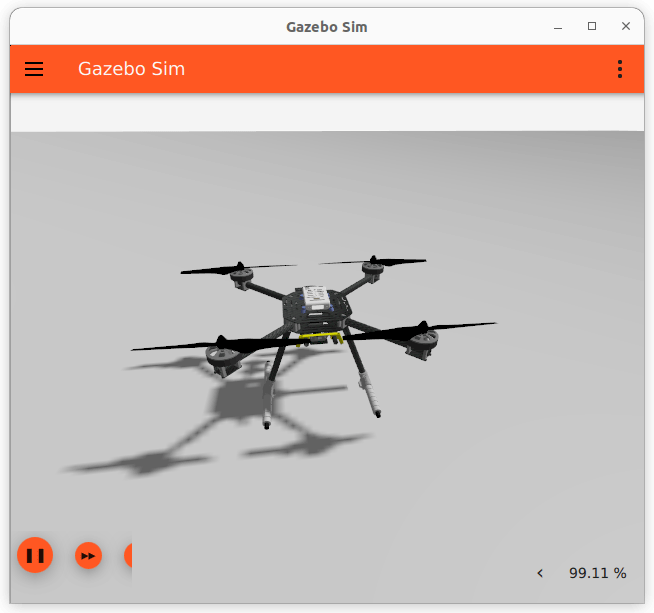
\includegraphics[height=0.42\textheight]{gazebo_x500}\\
    \credito{Gazebo con el x500. Documentación de PX4 (CC BY 4.0)}
  \end{columns}
  \vspace{0.2em}
  \begin{idea}
    \small En la terminal \textbf{kitty} cada programa sale en su propio panel. En otra terminal salen todos
    juntos, cada línea con el nombre del programa al inicio. \textbf{Ctrl+C} los para a todos.
  \end{idea}
\end{frame}

\begin{frame}[fragile]{Variantes de vespo up}
  \camino{6}
  \begin{lstlisting}[style=bash]
vespo up --sim --world plaza_show                # en otro mundo (los de x500_retos)
vespo up --sim --custom x500_lidar_2d            # con otro modelo de dron
vespo up --sim --world cueva --custom x500_lidar_2d
vespo up --sim --headless                        # sin ventana de Gazebo (mas ligero)
vespo simulate --show                            # que modelos y mundos hay
  \end{lstlisting}
  \begin{columns}[c]
    \column{0.32\textwidth}\centering
    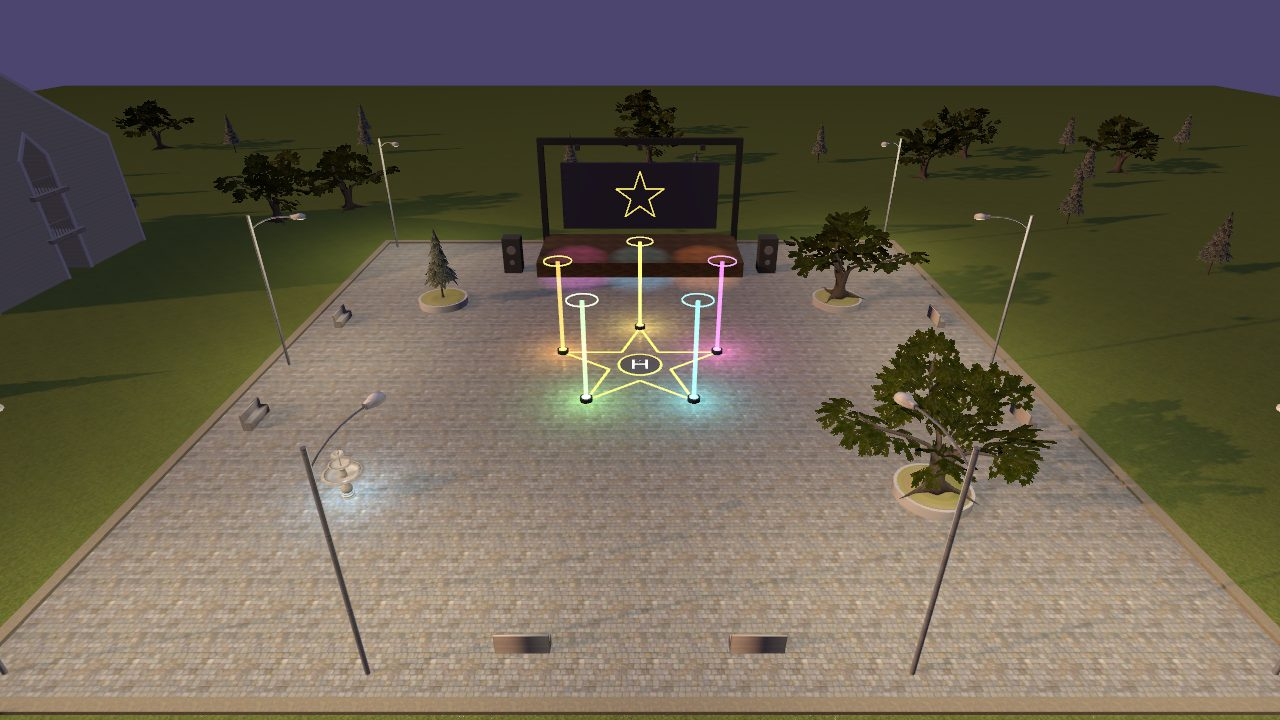
\includegraphics[width=\linewidth]{plaza_show}\\\credito{plaza\_show}
    \column{0.32\textwidth}\centering
    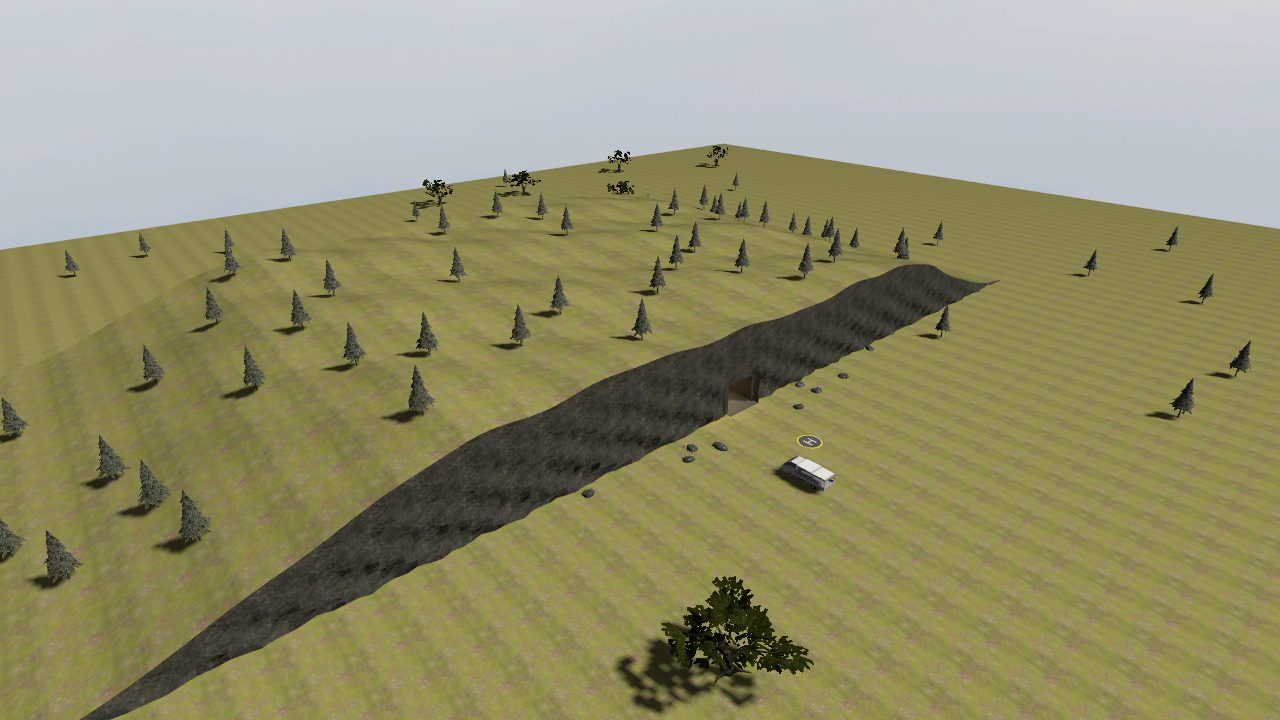
\includegraphics[width=\linewidth]{cueva}\\\credito{cueva}
    \column{0.32\textwidth}\centering
    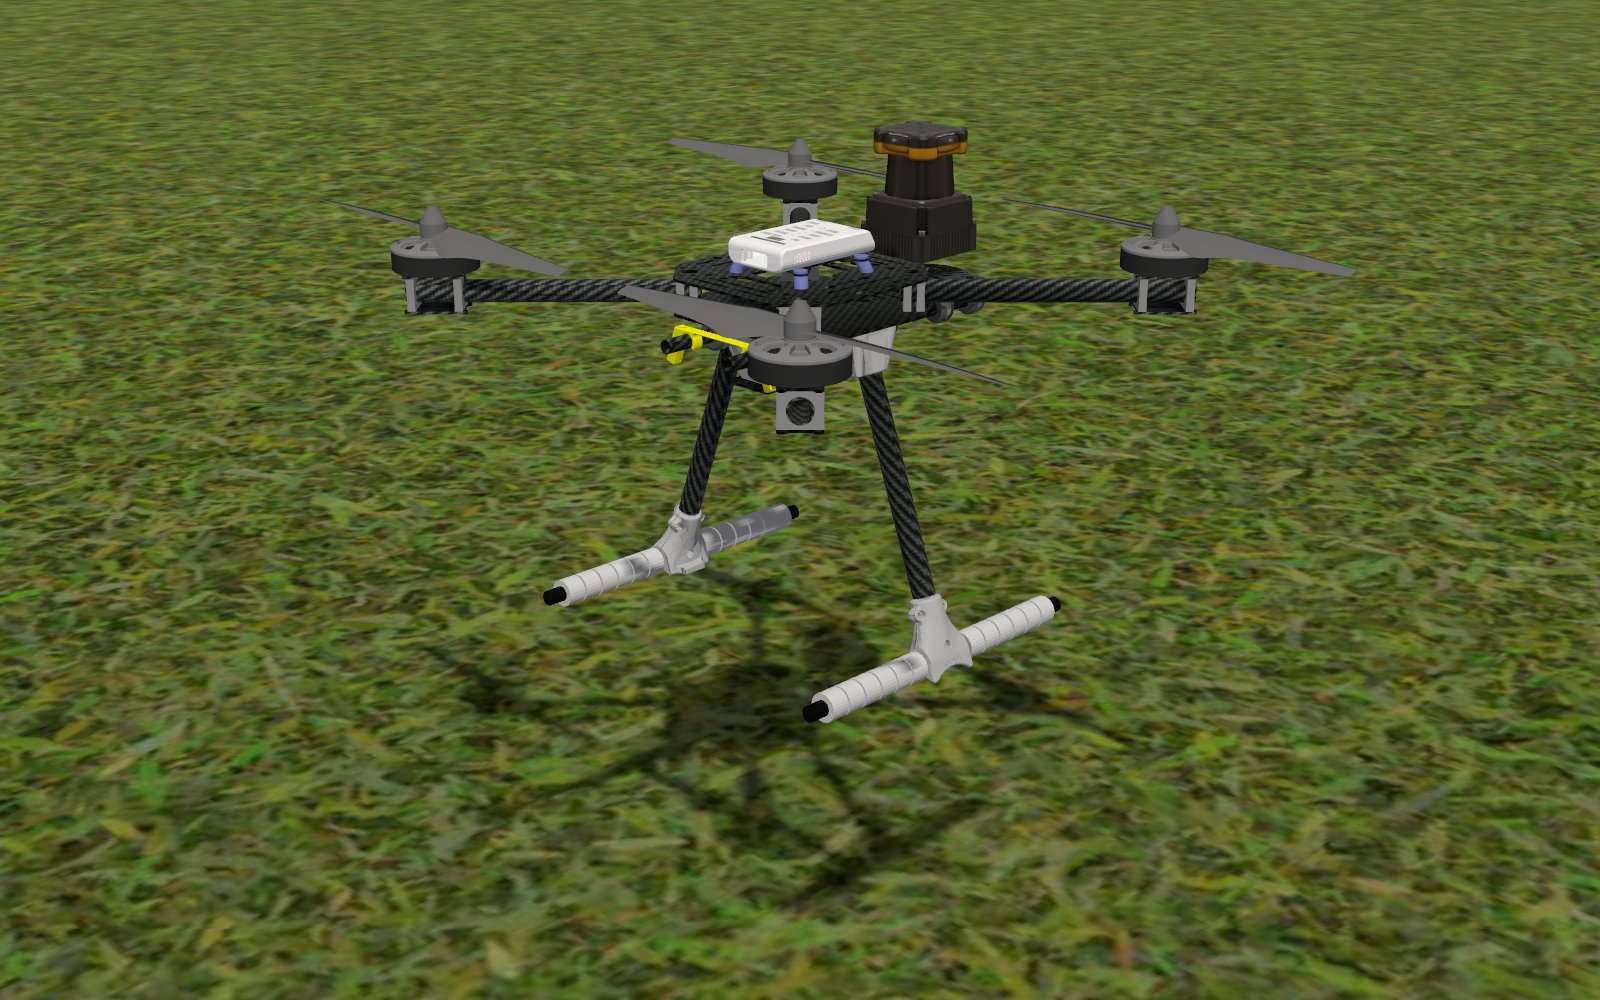
\includegraphics[width=\linewidth]{x500_lidar}\\\credito{x500\_lidar\_2d}
  \end{columns}
\end{frame}

\begin{frame}[fragile]{Paso 7: correr un ejemplo}
  \camino{7}
  \begin{columns}[c]
    \column{0.5\textwidth}
    \begin{lstlisting}[style=bash]
# en OTRA terminal (vespo up sigue corriendo)
ros2 run px4_examples telemetry_listener
    \end{lstlisting}
    \small
    \begin{itemize}
      \item \cmd{ros2 run \textit{paquete} \textit{programa}}.
      \item Tab completa los nombres: \cmd{ros2 run px4\_examples <Tab><Tab>} lista los 18 ejemplos.
      \item Lo paras con \textbf{Ctrl+C}.
    \end{itemize}
    \column{0.47\textwidth}
    \begin{terminal}{ros2 run px4\_examples telemetry\_listener}
Estado: desarmado | modo: HOLD (4)\\
Local: x=0.01 y=-0.02 alt=0.03 m\\
\ \ | vel=(0.00, 0.00, 0.00) m/s\\
GPS: lat=47.3979711 lon=8.5461637\\
Actitud: roll=0.1° pitch=-0.2° yaw=90.0°\\
Batería: 16.20 V | 100 \%
    \end{terminal}
    \small Si ves esto, \textbf{todo funciona}: ROS 2 ya habla con PX4.
  \end{columns}
\end{frame}

\begin{frame}[fragile]{Paso 8: apagar}
  \camino{8}
  \begin{columns}[c]
    \column{0.5\textwidth}
    \begin{lstlisting}[style=bash]
vespo down        # desde cualquier terminal
    \end{lstlisting}
    \small
    \begin{itemize}
      \item Para todo lo que levantó \cmd{vespo up}, y cualquier PX4, Gazebo o agente que haya quedado
        prendido.
      \item Úsalo también si la simulación se trabó: después \cmd{vespo up -{}-sim} otra vez.
    \end{itemize}
    \column{0.47\textwidth}
    \begin{ojo}[title={\small\bfseries Procesos zombis}]
      \small Si cierras la ventana de la terminal en vez de Ctrl+C, Gazebo o PX4 pueden quedarse corriendo
      escondidos. El siguiente \cmd{vespo up} choca con ellos (``port 8888 busy''). \cmd{vespo down} los
      limpia.
    \end{ojo}
  \end{columns}
\end{frame}

\begin{frame}[fragile]{El día a día}
  \begin{columns}[c]
    \column{0.55\textwidth}
    \begin{lstlisting}[style=bash]
vespo update                 # lo nuevo del equipo
vespo up --sim               # terminal 1
ros2 run px4_examples ...    # terminal 2
# ... editas un .cpp ...
vespo build px4_examples     # terminal 2
ros2 run px4_examples ...    # otra vez
vespo down                   # al terminar
    \end{lstlisting}
    \column{0.42\textwidth}\small
    \begin{itemize}
      \item \cmd{vespo} te \textbf{avisa solo} cuando el equipo subió algo nuevo.
      \item No hace falta reiniciar la simulación para probar otra versión de tu nodo: Ctrl+C al nodo,
        compilas y lo corres de nuevo.
      \item \cmd{vespo config}: ver la configuración de tu máquina.
    \end{itemize}
  \end{columns}
\end{frame}

% =============================================================================
\section{Repaso: el x500 y PX4}
% =============================================================================

\begin{frame}{El x500 en una lámina}
  \centering
  \begin{tikzpicture}
    \node[anchor=south west,inner sep=0] (img) at (0,0) {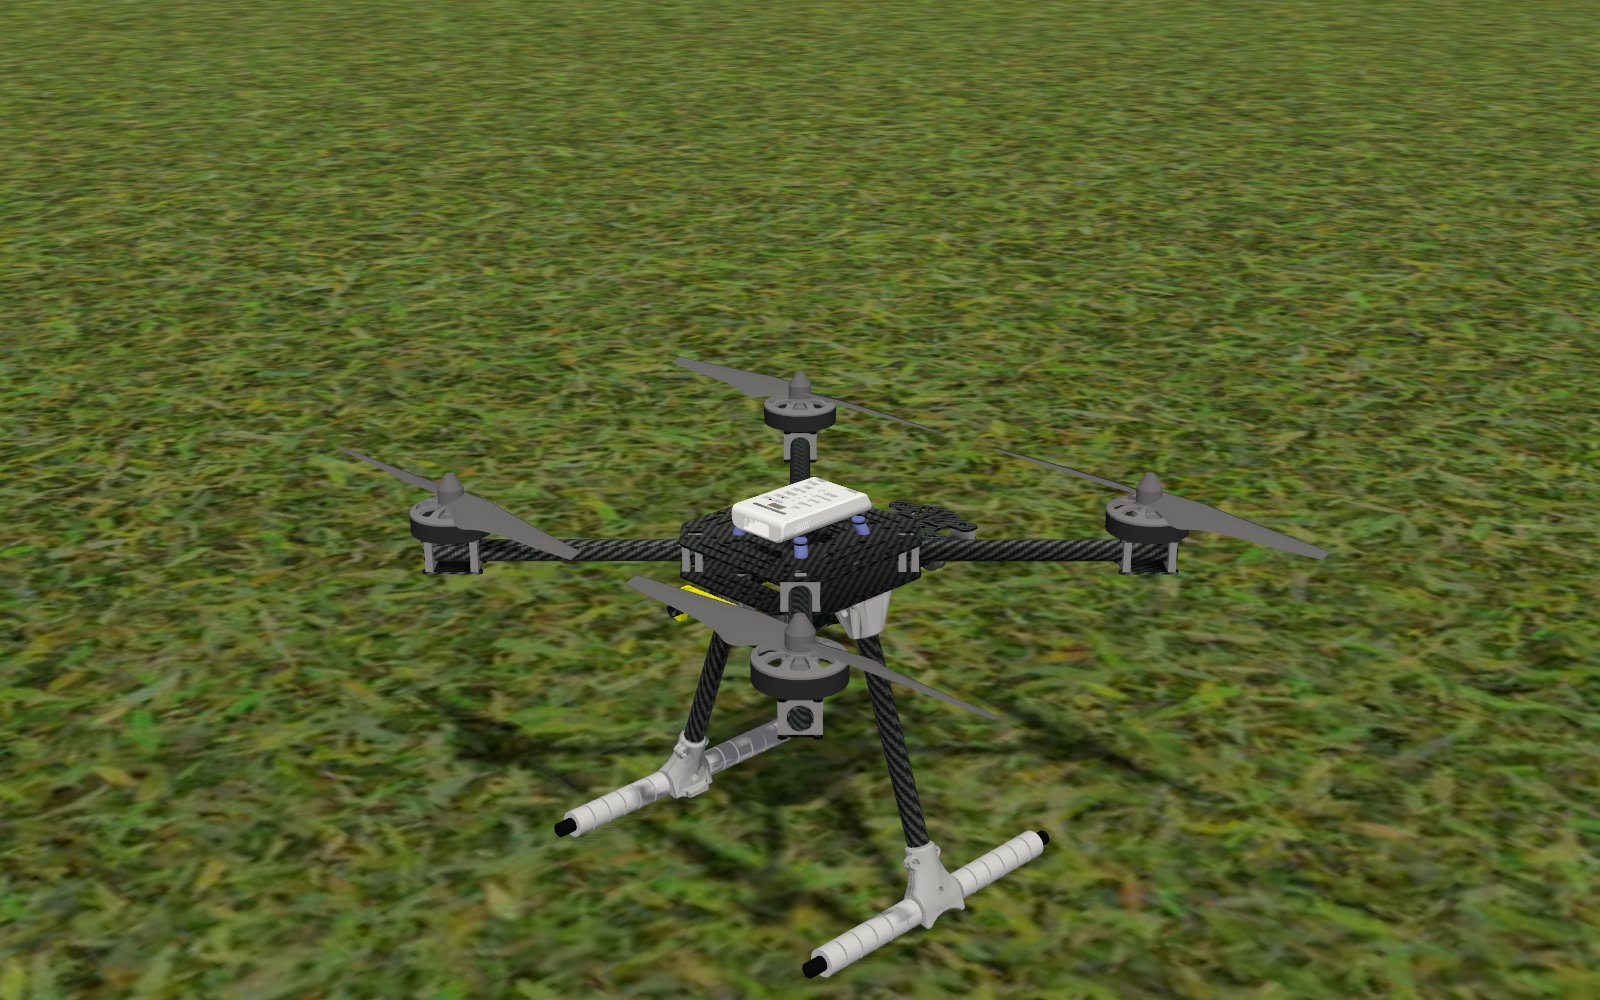
\includegraphics[height=0.78\textheight]{x500_tres_cuartos}};
    \begin{scope}[x={(img.south east)},y={(img.north west)},
        lb/.style={draw=azul,fill=white,rounded corners,font=\scriptsize,align=center,inner sep=2pt},
        fl/.style={-{Stealth},thick,azul}]
      \node[lb] (m) at (0.12,0.78) {\textbf{motor + hélice}\\4, uno por brazo};
      \draw[fl] (m) -- (0.28,0.50);
      \node[lb] (b) at (0.13,0.30) {\textbf{brazo}\\fibra de carbono};
      \draw[fl] (b) -- (0.36,0.44);
      \node[lb] (p) at (0.80,0.82) {\textbf{placa central}\\aquí va la Pixhawk (PX4)};
      \draw[fl] (p) -- (0.55,0.47);
      \node[lb] (t) at (0.85,0.22) {\textbf{tren de aterrizaje}};
      \draw[fl] (t) -- (0.60,0.12);
    \end{scope}
  \end{tikzpicture}\\
  \credito{El x500 de la simulación de PX4. Render propio de Gazebo}
\end{frame}

\begin{frame}{Cómo se mueve}
  \centering
  \begin{tikzpicture}[every node/.style={font=\scriptsize,align=center}]
    \foreach \x/\t/\d in {0/Subir/los 4 motores más rápido,3.6/Avanzar/se inclina hacia adelante:\\los de atrás más rápido,
        7.2/Ir a la derecha/se inclina a la derecha:\\los de la izquierda más rápido,10.8/Girar (yaw)/acelera un par diagonal\\y frena el otro} {
      \node at (\x,1.6) {\textbf{\t}};
      \node at (\x,0) {\dronarriba{2.1cm}};
      \node[text width=3.2cm] at (\x,-1.6) {\d};
    }
    % subir: 4 flechas hacia arriba (afuera de la página)
    \foreach \dx/\dy in {-0.55/0.55,0.55/0.55,-0.55/-0.55,0.55/-0.55} \fill[naranja] (\dx,\dy) circle (3.5pt);
    % avanzar: los de atrás
    \foreach \dx/\dy in {-0.55/-0.55,0.55/-0.55} \fill[naranja] (3.6+\dx,\dy) circle (3.5pt);
    \draw[-{Stealth},line width=2pt,verde] (3.6,0.4) -- (3.6,1.2);
    % derecha: los de la izquierda
    \foreach \dx/\dy in {-0.55/0.55,-0.55/-0.55} \fill[naranja] (7.2+\dx,\dy) circle (3.5pt);
    \draw[-{Stealth},line width=2pt,verde] (7.6,0) -- (8.5,0);
    % yaw: el par 1-2 (antihorario) más rápido -> el dron gira a la derecha
    \foreach \dx/\dy in {0.55/0.55,-0.55/-0.55} \fill[naranja] (10.8+\dx,\dy) circle (3.5pt);
    \draw[-{Stealth},line width=2pt,verde] (10.8,1.15) arc (90:20:1.15);
  \end{tikzpicture}
  \vspace{0.4em}

  \raggedright\small {\color{naranja}$\bullet$} = motor que acelera. El frente del dron es \textbf{arriba} en
  los dibujos. Nunca le dices a PX4 qué motor acelerar: le dices \textbf{a dónde ir} y él lo calcula.
\end{frame}

\begin{frame}{Los modos de vuelo: quién manda}
  \centering
  \begin{tikzpicture}[every node/.style={font=\scriptsize,align=center},
      md/.style={draw=azul,fill=azulclaro,rounded corners,text width=3.3cm,minimum height=1.45cm}]
    \node[md] at (0,1.0) {\textbf{Hold} \color{gris}(nav 4)\\\color{black}se queda quieto en el aire};
    \node[md,fill=yellow!25,draw=naranja] at (3.8,1.0) {\textbf{Offboard} \color{gris}(nav 14)\\\color{black}obedece a \textbf{tu nodo}};
    \node[md] at (7.6,1.0) {\textbf{Takeoff} \color{gris}(nav 17)\\\color{black}despega a una altura};
    \node[md] at (11.4,1.0) {\textbf{Land} \color{gris}(nav 18)\\\color{black}aterriza donde está};
    \node[md] at (0,-0.8) {\textbf{Return} \color{gris}(nav 5)\\\color{black}regresa a casa y aterriza};
    \node[md] at (3.8,-0.8) {\textbf{Position} \color{gris}(nav 2)\\\color{black}un piloto lo vuela\\con el control};
    \node[md] at (7.6,-0.8) {\textbf{Mission} \color{gris}(nav 3)\\\color{black}sigue waypoints\\hechos en QGC};
    \node[md] at (11.4,-0.8) {\textbf{Orbit} \color{gris}(nav 21)\\\color{black}da vueltas a un punto};
  \end{tikzpicture}
  \vspace{0.4em}

  \raggedright\small El modo actual sale en QGC y en \cmd{vehicle\_status\_v1.nav\_state}. Si tu nodo ``no hace
  nada'', lo primero es ver \textbf{en qué modo está}.
\end{frame}

\begin{frame}{Las reglas del piloto}
  \begin{columns}[c]
    \column{0.3\textwidth}\centering
    \dronlado{\linewidth}\\[0.4em]
    \small PX4 \textbf{siempre} está a cargo, aunque tu nodo esté mandando.
    \column{0.67\textwidth}\small
    \begin{enumerate}
      \item \textbf{No arma} si algo no está bien: sin GPS, con el estimador sin converger, sin
        QGroundControl conectado\ldots{} QGC dice la razón.
      \item \textbf{Armado} = motores girando. Si no despega en unos segundos, se \textbf{desarma solo}.
      \item En \textbf{Offboard}, si tu nodo deja de mandar mensajes \textasciitilde0.5 s, pasa a
        \textbf{Hold}.
      \item Con \textbf{batería baja} regresa a casa (Return) solo.
      \item Desde QGC \textbf{siempre} se le puede quitar el control a tu nodo: Hold, Land, Return.
    \end{enumerate}
  \end{columns}
\end{frame}

% =============================================================================
\section{Cómo habla ROS 2 con PX4}
% =============================================================================

\begin{frame}{Tres programas en fila}
  \centering
  \begin{tikzpicture}[every node/.style={font=\scriptsize,align=center}]
    \node (d) at (0,0) {\dronarriba{2.6cm}};
    \node[font=\small\bfseries] at (0,-1.7) {PX4};
    \node[font=\tiny,text=gris] at (0,-2.1) {(en la Pixhawk o en SITL)};
    \node[draw=azul,fill=azulclaro,rounded corners,minimum width=2.6cm,minimum height=1.4cm] (a) at (5,0)
      {\textbf{MicroXRCEAgent}\\el traductor};
    \node[draw=naranja,fill=yellow!25,rounded corners,minimum width=2.6cm,minimum height=1.4cm] (n) at (10,0)
      {\textbf{tu nodo}\\de ROS 2};
    \draw[-{Stealth},line width=1.5pt,verde] (1.6,0.35) -- node[above]{\cmd{/fmu/out/...}} (a.west |- 0,0.35);
    \draw[{Stealth}-,line width=1.5pt,naranja] (1.6,-0.35) -- node[below]{\cmd{/fmu/in/...}} (a.west |- 0,-0.35);
    \draw[-{Stealth},line width=1.5pt,verde] (a.east |- 0,0.35) -- node[above]{telemetría} (n.west |- 0,0.35);
    \draw[{Stealth}-,line width=1.5pt,naranja] (a.east |- 0,-0.35) -- node[below]{órdenes} (n.west |- 0,-0.35);
    \node[font=\tiny,text=gris] at (2.6,1.5) {UDP 8888 (sim)\\o cable serial (real)};
    \node[font=\tiny,text=gris] at (7.5,1.5) {topics de ROS 2};
  \end{tikzpicture}
  \vspace{0.6em}

  \raggedright\small
  \begin{itemize}
    \item PX4 no habla ROS 2 directamente: el \textbf{agente} traduce. \cmd{vespo up} lo arranca solo.
    \item \textbf{Sin agente no existe ningún topic} \cmd{/fmu/...} en ROS 2.
    \item \cmd{out}: PX4 te cuenta (\textcolor{verde}{verde}). \cmd{in}: tú le pides (\textcolor{naranja}{naranja}).
  \end{itemize}
\end{frame}

\begin{frame}{El mapa de topics}
  \centering
  \begin{tikzpicture}[every node/.style={font=\scriptsize,align=center},
      o/.style={draw=verde,fill=verdeclaro,rounded corners,text width=3.6cm,minimum height=0.7cm},
      i/.style={draw=naranja,fill=yellow!20,rounded corners,text width=3.6cm,minimum height=0.7cm}]
    \node (d) at (0,0) {\dronarriba{2.4cm}};
    \node[o] (o1) at (-4.8,2.0) {\cmd{vehicle\_status\_v1}\\¿armado? ¿qué modo?};
    \node[o] (o2) at (-4.8,0.65) {\cmd{vehicle\_local\_position\_v1}\\dónde está, en metros};
    \node[o] (o3) at (-4.8,-0.7) {\cmd{vehicle\_global\_position}\\latitud, longitud};
    \node[o] (o4) at (-4.8,-2.05) {\cmd{vehicle\_attitude}\\hacia dónde apunta};
    \node[o] (o5) at (4.8,2.0) {\cmd{battery\_status\_v1}\\voltaje y \%};
    \node[o] (o6) at (4.8,0.75) {\cmd{vehicle\_command\_ack}\\¿aceptó mi comando?};
    \node[i] (i1) at (4.8,-0.6) {\cmd{offboard\_control\_mode}\\``sigo vivo'' (heartbeat)};
    \node[i] (i2) at (4.8,-1.6) {\cmd{trajectory\_setpoint}\\a dónde ir};
    \node[i] (i3) at (4.8,-2.6) {\cmd{vehicle\_command}\\armar, despegar, aterrizar\ldots};
    \foreach \n in {o1,o2,o3,o4} \draw[-{Stealth},thick,verde] (d) -- (\n.east);
    \foreach \n in {o5,o6} \draw[-{Stealth},thick,verde] (d) -- (\n.west);
    \foreach \n in {i1,i2,i3} \draw[-{Stealth},thick,naranja] (\n.west) -- (d);
  \end{tikzpicture}
  \vspace{0.2em}

  \raggedright\small Todos empiezan con \cmd{/fmu/out/} (verde) o \cmd{/fmu/in/} (naranja). Con estos
  nueve se hacen los 18 ejemplos.
\end{frame}

\begin{frame}{La trampa del \_v1}
  \begin{columns}[c]
    \column{0.5\textwidth}\centering
    \begin{tikzpicture}[every node/.style={font=\scriptsize,align=center}]
      \node[draw=azul,fill=azulclaro,rounded corners] (p) at (0,0) {PX4 transmite en\\\cmd{vehicle\_status\_v1}};
      \foreach \r in {0.4,0.7,1.0} \draw[naranja,thick] (1.25,0) ++(-40:\r) arc (-40:40:\r);
      \node[draw=verde,fill=verdeclaro,rounded corners] at (4.4,0.9) {sintonizas\\\cmd{vehicle\_status\_v1}\\\color{verde}\bfseries te llega};
      \node[draw=rojo,fill=red!5,rounded corners] at (4.4,-0.9) {sintonizas\\\cmd{vehicle\_status}\\\color{rojo}\bfseries silencio};
    \end{tikzpicture}
    \column{0.47\textwidth}\small
    \begin{itemize}
      \item Cuando PX4 cambia un mensaje, el nombre del topic cambia: \cmd{\_v1}, \cmd{\_v2}\ldots
      \item Si te equivocas de nombre \textbf{no sale ningún error}: tu nodo se queda esperando para siempre.
      \item Copia los nombres de los ejemplos, o de\\\cmd{ros2 topic list | grep fmu}.
    \end{itemize}
  \end{columns}
\end{frame}

\begin{frame}{QoS: radio en vivo o carta certificada}
  \begin{columns}[c]
    \column{0.5\textwidth}
    \begin{idea}[title={\small\bfseries best\_effort = radio en vivo},coltitle=black,colbacktitle=azulclaro]
      \small Si un mensaje se pierde, ya pasó: el siguiente llega en milisegundos. \textbf{Así publica PX4}.
    \end{idea}
    \begin{idea}[title={\small\bfseries reliable = carta certificada},coltitle=black,colbacktitle=azulclaro]
      \small Se reenvía hasta que llega. Es lo que usa ROS 2 si no dices nada.
    \end{idea}
    \column{0.47\textwidth}\centering\small
    \begin{tabular}{llc}
      \toprule
      PX4 publica & tu nodo pide & ¿llega? \\
      \midrule
      best\_effort & best\_effort & \ok \\
      best\_effort & reliable & \mal \\
      \bottomrule
    \end{tabular}
    \vspace{0.6em}

    \raggedright Por eso todos los ejemplos empiezan con:\\[0.2em]
    \cmd{\scriptsize auto qos = rclcpp::QoS(1)}\\
    \cmd{\scriptsize\ \ .best\_effort().transient\_local();}
  \end{columns}
\end{frame}

\begin{frame}[fragile]{Espiar desde la terminal}
  \small Con \cmd{vespo up -{}-sim} corriendo, sin escribir código:
  \begin{lstlisting}[style=bash]
ros2 topic list | grep fmu                                   # que publica PX4
ros2 topic echo /fmu/out/vehicle_status_v1 --field nav_state  # el modo, en vivo
ros2 topic hz /fmu/out/vehicle_local_position_v1             # cada cuanto llega
ros2 interface show px4_msgs/msg/TrajectorySetpoint          # los campos de un mensaje
  \end{lstlisting}
  \begin{columns}[c]
    \column{0.45\textwidth}
    \begin{terminal}{ros2 topic echo ... --field nav\_state}
4\\
---\\
14\\
---
    \end{terminal}
    \column{0.52\textwidth}\small
    Cambia el modo desde QGC y míralo cambiar: \textbf{4} = Hold, \textbf{14} = Offboard, \textbf{18} = Land.
    Es la forma más rápida de saber si PX4 te está haciendo caso.
  \end{columns}
\end{frame}

% =============================================================================
\section{shared\_ptr: lo único de C++ que hoy hace falta}
% =============================================================================

\begin{frame}{El problema: un mensaje, muchos interesados}
  \begin{columns}[c]
    \column{0.52\textwidth}\centering
    \begin{tikzpicture}[every node/.style={font=\scriptsize,align=center}]
      \node (d) at (0,0) {\dronarriba{1.6cm}};
      \node[draw=gray,fill=yellow!15,rounded corners,minimum width=1.9cm,minimum height=1cm] (m) at (2.8,0)
        {un mensaje\\\cmd{VehicleStatus}};
      \draw[-{Stealth},thick,verde] (d) -- (m);
      \foreach \y/\n/\k in {1.3/telemetry\_listener/a,0/tu misión/b,-1.3/battery\_monitor/c} {
        \node[draw=azul,fill=azulclaro,rounded corners] (n\k) at (6.2,\y) {\n};
        \draw[-{Stealth},thick] (m) -- (n\k.west);}
    \end{tikzpicture}
    \column{0.45\textwidth}\small
    \begin{itemize}
      \item Llega un mensaje y lo quieren \textbf{varias} partes del programa.
      \item ¿Copiarlo para cada una? Lento.
      \item ¿Compartir el original? Entonces, \textbf{¿quién lo borra} y cuándo? Si se borra antes de tiempo,
        el programa truena; si nadie lo borra, se acaba la memoria.
    \end{itemize}
  \end{columns}
\end{frame}

\begin{frame}{Primero: un apuntador es una dirección}
  \begin{columns}[c]
    \column{0.5\textwidth}\centering
    \begin{tikzpicture}[every node/.style={font=\scriptsize,align=center}]
      \draw[fill=yellow!15,rounded corners] (3,0) rectangle (5.4,1.5);
      \node at (4.2,1.1) {\textbf{la casa}};
      \node at (4.2,0.5) {(el mensaje)};
      \node[below,font=\tiny] at (4.2,0) {Calle Dron 14};
      \draw[fill=azulclaro,rounded corners] (0,0.35) rectangle (2,1.15);
      \node at (1,0.75) {papelito:\\``Calle Dron 14''};
      \node[below,font=\tiny] at (1,0.35) {el apuntador};
      \draw[-{Stealth},thick,rojo] (2,0.75) -- (3,0.75);
    \end{tikzpicture}
    \column{0.47\textwidth}\small
    \begin{itemize}
      \item El mensaje vive en un lugar de la memoria (la \textbf{casa}).
      \item Un \textbf{apuntador} es un papelito con la dirección. Copiar el papelito es barato; copiar la
        casa no.
      \item \cmd{msg->nav\_state}: ve a esa dirección y lee \cmd{nav\_state}.
      \item \cmd{*msg}: la casa completa.
    \end{itemize}
  \end{columns}
\end{frame}

\begin{frame}[fragile]{shared\_ptr: la casa que se borra sola}
  \begin{columns}[c]
    \column{0.5\textwidth}\centering
    \begin{tikzpicture}[every node/.style={font=\scriptsize,align=center}]
      \draw[alt=<6>{fill=gray!20,draw=gray}{fill=yellow!15}, rounded corners] (3,-0.6) rectangle (5.6,1.4);
      \node at (4.3,1.0) {\textbf{mensaje}};
      \node[alt=<6>{text=gris}{}] at (4.3,0.4) {\only<1,5>{dueños: \textbf{1}}\only<2,4>{dueños: \textbf{2}}\only<3>{dueños: \textbf{3}}\only<6>{dueños: \textbf{0}}};
      \node[font=\scriptsize\bfseries,text=rojo,visible on=<6>] at (4.3,-0.2) {¡borrado!};
      \node[draw=azul,fill=azulclaro,rounded corners,minimum width=1.5cm,alt=<1-5>{}{invisible}] (a) at (0.6,1.2) {\cmd{a}};
      \node[draw=azul,fill=azulclaro,rounded corners,minimum width=1.5cm,visible on=<2-4>] (b) at (0.6,0.4) {\cmd{b}};
      \node[draw=azul,fill=azulclaro,rounded corners,minimum width=1.5cm,visible on=<3>] (c) at (0.6,-0.4) {\cmd{c}};
      \draw[-{Stealth},thick,visible on=<1-5>] (a) -- (3,0.8);
      \draw[-{Stealth},thick,visible on=<2-4>] (b) -- (3,0.4);
      \draw[-{Stealth},thick,visible on=<3>] (c) -- (3,0);
    \end{tikzpicture}
    \column{0.47\textwidth}
    \begin{lstlisting}[style=cpp,escapechar=!]
auto a = std::make_shared<VehicleStatus>();  !\only<1>{\textcolor{rojo}{$\blacktriangleleft$}}!
{
  auto b = a;     // copia el papelito  !\only<2>{\textcolor{rojo}{$\blacktriangleleft$}}!
  {
    auto c = a;  !\only<3>{\textcolor{rojo}{$\blacktriangleleft$}}!
  }  // c deja de existir  !\only<4>{\textcolor{rojo}{$\blacktriangleleft$}}!
}    // b deja de existir  !\only<5>{\textcolor{rojo}{$\blacktriangleleft$}}!
// a deja de existir: nadie lo usa  !\only<6>{\textcolor{rojo}{$\blacktriangleleft$}}!
    \end{lstlisting}
    \small
    \only<1>{Se crea el mensaje. Una variable lo apunta: \textbf{1 dueño}.}%
    \only<2>{Copiar un \cmd{shared\_ptr} copia la dirección, no el mensaje. Ahora son \textbf{2}.}%
    \only<3>{Otro más: \textbf{3} dueños. Los tres ven el \textbf{mismo} mensaje.}%
    \only<4>{Cuando \cmd{c} sale de sus llaves, deja de existir y la cuenta baja.}%
    \only<5>{Lo mismo con \cmd{b}.}%
    \only<6>{El último dueño desaparece: la cuenta llega a 0 y el mensaje \textbf{se borra solo}. Nadie tuvo que
      acordarse.}%
  \end{columns}
\end{frame}

\begin{frame}{Por eso en ROS 2 todo es SharedPtr}
  \centering
  \begin{tikzpicture}[every node/.style={font=\scriptsize,align=center},
      bx/.style={draw=azul,fill=azulclaro,rounded corners,text width=3.2cm,minimum height=1.25cm}]
    \node[bx] at (0,0) {\textbf{Los mensajes}\\\cmd{VehicleStatus::SharedPtr msg}\\se entregan sin copiar};
    \node[bx] at (4.2,0) {\textbf{El nodo}\\\cmd{std::make\_shared<Nodo>()}\\vive mientras gira};
    \node[bx] at (8.4,0) {\textbf{Publishers, subs, timers}\\\cmd{...::SharedPtr pub\_}\\existen mientras los guardes};
  \end{tikzpicture}
  \vspace{0.6em}

  \begin{idea}
    \small \cmd{VehicleStatus::SharedPtr} es solo otro nombre para \cmd{std::shared\_ptr<VehicleStatus>}. Cuando
    lo veas, piensa: ``un papelito con la dirección de un \cmd{VehicleStatus}''.
  \end{idea}
\end{frame}

\begin{frame}[fragile]{En los ejemplos: guardar una copia con *msg}
  \begin{lstlisting}[style=cpp,escapechar=!]
VehicleStatus status_;                       // !\textbf{la última copia}!, para usarla después

status_sub_ = create_subscription<VehicleStatus>(
  "/fmu/out/vehicle_status_v1", qos,
  [this](const VehicleStatus::SharedPtr msg) {   // msg = el papelito
    status_ = *msg;                              // *msg = el mensaje: se copia
  });
  \end{lstlisting}
  \centering
  \begin{tikzpicture}[every node/.style={font=\scriptsize,align=center}]
    \node[draw=azul,fill=azulclaro,rounded corners] (m) at (0,0) {\cmd{msg}\\(SharedPtr)};
    \node[draw=gray,fill=yellow!15,rounded corners] (x) at (3.2,0) {mensaje que llegó\\(se borra al salir)};
    \node[draw=verde,fill=verdeclaro,rounded corners] (s) at (7.2,0) {\cmd{status\_}\\copia que se queda};
    \draw[-{Stealth},thick] (m) -- (x);
    \draw[-{Stealth},thick,verde] (x) -- node[above]{\cmd{status\_ = *msg}} (s);
  \end{tikzpicture}
  \vspace{0.3em}

  \raggedright\small El callback \textbf{guarda}; el timer, cada 100 ms, \textbf{decide} con lo último que
  guardó. Así están hechos todos los ejemplos.
\end{frame}

\begin{frame}[fragile]{El error clásico: la suscripción que se muere}
  \begin{columns}[t]
    \column{0.48\textwidth}
    \begin{ojo}[title={\small\bfseries MAL: nunca recibe nada}]
      \begin{lstlisting}[style=cpp,frame=none]
Nodo() : Node("nodo") {
  auto sub = create_subscription<...>(...);
}  // sub era local: aqui se borra
   // y la suscripcion con el
      \end{lstlisting}
    \end{ojo}
    \column{0.48\textwidth}
    \begin{idea}[title={\small\bfseries BIEN: como en los ejemplos},coltitle=black,colbacktitle=azulclaro]
      \begin{lstlisting}[style=cpp,frame=none]
rclcpp::Subscription<...>::SharedPtr sub_;
Nodo() : Node("nodo") {
  sub_ = create_subscription<...>(...);
}  // sub_ es del nodo: vive con el
      \end{lstlisting}
    \end{idea}
  \end{columns}
  \vspace{0.3em}
  \small Es el \cmd{shared\_ptr} en acción: cuando el último dueño desaparece, el objeto se borra. Guarda
  publishers, subscriptions y timers en variables \textbf{del nodo} (las que terminan en \cmd{\_}).
\end{frame}

\begin{frame}{Resumen: punto, flecha y asterisco}
  \centering\small
  \begin{tabular}{lll}
    \toprule
    Escribes & Cuando tienes & Significa \\
    \midrule
    \cmd{status\_.nav\_state} & un mensaje (\cmd{VehicleStatus}) & el campo, directo \\
    \cmd{msg->nav\_state} & un apuntador (\cmd{SharedPtr}) & ve a la dirección y lee el campo \\
    \cmd{*msg} & un apuntador & el mensaje completo \\
    \cmd{pub\_->publish(m)} & un publisher (\cmd{SharedPtr}) & llamar una función a través del apuntador \\
    \bottomrule
  \end{tabular}
  \vspace{0.6em}

  \raggedright\small Regla rápida: si la variable es un \cmd{SharedPtr}, usa \cmd{->}; si es el objeto,
  usa \cmd{.}. El compilador te avisa si te equivocas.
\end{frame}

% =============================================================================
\section{Escuchar al dron}
% =============================================================================

\begin{frame}{Todos los que escuchan tienen la misma forma}
  \centering
  \begin{tikzpicture}[every node/.style={font=\scriptsize,align=center},
      bx/.style={draw=azul,fill=azulclaro,rounded corners,minimum height=1cm,text width=2.4cm}]
    \node (d) at (0,0) {\dronarriba{1.8cm}};
    \node[bx] (cb) at (3.4,0) {\textbf{callbacks}\\guardan: \cmd{status\_ = *msg}};
    \node[bx,fill=yellow!20] (m) at (6.9,0) {\textbf{variables del nodo}\\\cmd{status\_}, \cmd{position\_}\ldots};
    \node[bx] (t) at (10.4,0) {\textbf{timer} (1 Hz)\\lee e imprime};
    \node[draw=verde,fill=verdeclaro,rounded corners,font=\ttfamily\tiny] (o) at (10.4,-1.7) {Estado: armado | modo: \ldots};
    \draw[-{Stealth},thick,verde] (d) -- node[above,font=\tiny]{cuando llega} (cb);
    \draw[-{Stealth},thick] (cb) -- (m);
    \draw[-{Stealth},thick] (m) -- (t);
    \draw[-{Stealth},thick] (t) -- (o);
  \end{tikzpicture}
  \vspace{0.5em}

  \raggedright\small
  \begin{itemize}
    \item Los mensajes llegan a 50--250 Hz: si imprimes en el callback, la terminal se vuelve ilegible.
    \item Por eso el callback solo \textbf{guarda} y un timer \textbf{imprime} una vez por segundo.
    \item Ninguno de estos nodos manda órdenes: son seguros de correr \textbf{siempre}, incluso con el dron real.
  \end{itemize}
\end{frame}

\begin{frame}{telemetry\_listener: todo de un vistazo}
  \begin{columns}[c]
    \column{0.5\textwidth}
    \begin{terminal}{ros2 run px4\_examples telemetry\_listener}
Estado: armado | modo: OFFBOARD (14)\\
Local: x=4.98 y=0.02 alt=5.01 m\\
\ \ | vel=(0.01, 1.98, 0.00) m/s\\
GPS: lat=47.3980159 lon=8.5461640\\
\ \ alt=5.1 m (AMSL)\\
Actitud: roll=2.1° pitch=0.4° yaw=0.2°\\
Batería: 15.40 V | 71 \%
    \end{terminal}
    \credito{Ejemplo durante \cmd{square\_mission}, yendo al este.}
    \column{0.47\textwidth}\small
    \begin{tabular}{@{}ll@{}}
      \textbf{Estado} & \cmd{vehicle\_status\_v1} \\
      \textbf{Local} & \cmd{vehicle\_local\_position\_v1} \\
      \textbf{GPS} & \cmd{vehicle\_global\_position} \\
      \textbf{Actitud} & \cmd{vehicle\_attitude} \\
      \textbf{Batería} & \cmd{battery\_status\_v1} \\
    \end{tabular}
    \vspace{0.6em}
    \begin{idea}
      \small Pruébalo: con el dron en el aire, \textbf{muévelo desde QGC} y mira cómo cambian \cmd{x},
      \cmd{y}, \cmd{alt} y el \cmd{yaw}. Así se aprende NED sin fórmulas.
    \end{idea}
  \end{columns}
\end{frame}

\begin{frame}{Leer las coordenadas: NED}
  \begin{columns}[c]
    \column{0.45\textwidth}\centering
    \begin{tikzpicture}
      \draw[gray!30,step=0.6] (-0.3,-0.3) grid (3.3,3.3);
      \draw[-{Stealth},thick,verde] (0,0) -- (0,3.3) node[above,font=\scriptsize] {x = Norte};
      \draw[-{Stealth},thick,rojo] (0,0) -- (3.3,0) node[right,font=\scriptsize] {y = Este};
      \node[font=\tiny,below left] at (0,0) {(0,0) despegue};
      \node at (1.8,2.4) {\dronarriba{1.1cm}};
      \draw[dashed,gray] (1.8,0) -- (1.8,2.4) -- (0,2.4);
      \node[font=\tiny,left] at (0,2.4) {x=4};
      \node[font=\tiny,below] at (1.8,0) {y=3};
    \end{tikzpicture}
    \column{0.52\textwidth}\small
    \begin{itemize}
      \item \cmd{x}: metros al \textbf{norte} del despegue.
      \item \cmd{y}: metros al \textbf{este}.
      \item \cmd{z}: metros hacia \textbf{abajo}. Volando a 5 m, \cmd{z = -5}. Por eso los ejemplos imprimen
        \cmd{alt = -z}.
      \item \cmd{yaw}: hacia dónde apunta la nariz. 0° = norte, 90° = este.
    \end{itemize}
    \begin{ojo}
      \small En Gazebo los ejes son otros (x al este, z arriba). Lo que importa para tu nodo es NED.
    \end{ojo}
  \end{columns}
\end{frame}

\begin{frame}{flight\_mode\_monitor: el narrador}
  \begin{columns}[c]
    \column{0.45\textwidth}
    \begin{terminal}{ros2 run px4\_examples flight\_mode\_monitor}
DESARMADO\\
Modo: Hold\\
Chequeos de pre-vuelo: OK, se puede armar\\
ARMADO\\
Modo: Hold -> Offboard\\
Modo: Offboard -> Hold\\
FAILSAFE ACTIVO (modo Hold)\\
Banderas de failsafe:\\
\ \ señal offboard perdida
    \end{terminal}
    \column{0.52\textwidth}\centering
    \begin{tikzpicture}[every node/.style={font=\scriptsize,align=center},
        md/.style={draw=azul,fill=azulclaro,rounded corners,minimum width=1.6cm,minimum height=0.7cm}]
      \node[md] (h) at (0,0) {Hold};
      \node[md,fill=yellow!25] (o) at (2.6,0) {Offboard};
      \node[md,fill=red!10,draw=rojo] (f) at (5.2,0) {Hold\\(failsafe)};
      \draw[-{Stealth},thick] (h) -- node[above,font=\tiny]{tu nodo} (o);
      \draw[-{Stealth},thick,rojo] (o) -- node[above,font=\tiny]{Ctrl+C} (f);
    \end{tikzpicture}
    \vspace{0.6em}

    \raggedright\small Solo imprime cuando \textbf{algo cambia}: armado, modo, failsafe. Déjalo corriendo en una
    terminal \textbf{siempre} que pruebes algo: te dice qué hizo PX4 y por qué.
  \end{columns}
\end{frame}

\begin{frame}{battery\_monitor: tu propio failsafe}
  \begin{columns}[c]
    \column{0.42\textwidth}\centering
    \begin{tikzpicture}
      \draw[thick,rounded corners=2pt] (0,0) rectangle (1.4,3.2);
      \fill[gray] (0.45,3.2) rectangle (0.95,3.4);
      \fill[verde!70] (0.08,0.08) rectangle (1.32,2.2);
      \draw[rojo,line width=1.5pt] (-0.3,1.28) -- (1.7,1.28) node[right,font=\scriptsize,text=rojo] {\cmd{low\_percent}: 40 \%};
      \node[font=\scriptsize\bfseries] at (0.7,1.7) {71 \%};
      \node[font=\scriptsize,right,align=left] at (1.7,2.4) {arriba: \textbf{OK}};
      \node[font=\scriptsize,right,align=left] at (1.7,0.5) {abajo: \textbf{acción}\\\cmd{warn}, \cmd{land} o \cmd{rtl}};
    \end{tikzpicture}
    \column{0.55\textwidth}
    \begin{terminal}{battery\_monitor -p low\_percent:=40.0 -p action:=rtl}
85.0 \% | 15.80 V (3.95 V/celda, 4S)\\
\ \ | -1.0 A | OK\\
BATERÍA BAJA: 39.8 \% (umbral 40 \%)\\
Regresando a casa (RTL)
    \end{terminal}
    \small
    \begin{itemize}
      \item Escucha \cmd{battery\_status\_v1} y, bajo el umbral, \textbf{manda un comando} a PX4.
      \item En SITL la batería se descarga \textbf{rapidísimo} a propósito (\textasciitilde50 \% en medio
        minuto armado) para poder probar esto.
    \end{itemize}
  \end{columns}
\end{frame}

\begin{frame}[fragile]{Los cinco que escuchan}
  \centering\small
  \begin{tabular}{lll}
    \toprule
    Ejemplo & Escucha & Para qué \\
    \midrule
    \cmd{telemetry\_listener} & estado, posición, GPS, actitud, batería & ver todo de un vistazo \\
    \cmd{flight\_mode\_monitor} & estado, failsafes & saber qué hizo PX4 y por qué \\
    \cmd{battery\_monitor} & batería & actuar con batería baja \\
    \cmd{imu\_listener} & \cmd{sensor\_combined} & giroscopio y acelerómetro crudos \\
    \cmd{gps\_status} & \cmd{vehicle\_gps\_position} & satélites, precisión, ¿listo para volar? \\
    \bottomrule
  \end{tabular}
  \vspace{0.6em}

  \raggedright
  \begin{lstlisting}[style=bash]
ros2 run px4_examples imu_listener      # quieto marca z = -9.8: la gravedad
ros2 run px4_examples gps_status
  \end{lstlisting}
\end{frame}

% =============================================================================
\section{Volar en offboard}
% =============================================================================

\begin{frame}{La receta de offboard: tres ingredientes}
  \centering
  \begin{tikzpicture}[every node/.style={font=\scriptsize,align=center},
      ig/.style={draw=azul,fill=azulclaro,rounded corners,text width=3.4cm,minimum height=2.5cm}]
    \node[ig] (a) at (0,0) {\textbf{\large 1}\\[0.2em]\textbf{Heartbeat}\\\cmd{offboard\_control\_mode}\\[0.3em]``sigo vivo y voy a\\controlar por posición''\\[0.2em]\color{azul}10 veces por segundo};
    \node[ig] (b) at (4.2,0) {\textbf{\large 2}\\[0.2em]\textbf{Setpoint}\\\cmd{trajectory\_setpoint}\\[0.3em]``quiero estar en\\$(x, y, z)$ mirando a yaw''\\[0.2em]\color{azul}10 veces por segundo};
    \node[ig,fill=yellow!25] (c) at (8.4,0) {\textbf{\large 3}\\[0.2em]\textbf{Modo + armar}\\\cmd{vehicle\_command}\\[0.3em]``entra a Offboard''\\``arma los motores''\\[0.2em]\color{azul}una vez, tras 1 s};
    \node at (11.6,0) {\dronlado{2.2cm}};
    \node[font=\large] at (2.1,0) {+}; \node[font=\large] at (6.3,0) {+};
    \draw[-{Stealth},line width=1.5pt] (10.2,0) -- (10.6,0);
  \end{tikzpicture}
  \vspace{0.6em}

  \raggedright\small
  \begin{itemize}
    \item Sin \textbf{1} y \textbf{2} corriendo \textbf{antes}, PX4 rechaza entrar a Offboard: por eso el nodo ``calienta'' 1 s.
    \item Si \textbf{1} y \textbf{2} se detienen en pleno vuelo, PX4 pasa a Hold (failsafe).
    \item Los cinco ejemplos de offboard siguen esta receta; solo cambia \textbf{qué setpoint} mandan.
  \end{itemize}
\end{frame}

% -----------------------------------------------------------------------------
\begin{frame}{takeoff\_mission paso a paso}
  \begin{columns}[c]
    \column{0.42\textwidth}\centering
    \begin{tikzpicture}[scale=0.62]
      \fill[green!35!black!40] (-3,-0.25) rectangle (3,0);
      \draw[gray!50] (-2.6,0) -- (-2.6,6);
      \foreach \h in {0,1,...,6} \draw[gray!50] (-2.7,\h) -- (-2.5,\h) node[left,font=\tiny,text=gris] {\h\,m};
      \draw[dashed,rojo,thick] (-2.4,5) -- (2.8,5) node[above left,font=\tiny,text=rojo] {setpoint: z = $-5$};
      \only<1-2>{\node[anchor=south] at (0,0) {\dronlado{2.2cm}};}
      \only<3>{\node[anchor=south] at (0,2.4) {\dronlado{2.2cm}}; \draw[-{Stealth},line width=2pt,verde] (1.8,1.4) -- (1.8,3.6);}
      \only<4-5>{\node[anchor=south] at (0,4.55) {\dronlado{2.2cm}};}
      \only<2>{\foreach \x in {-1.25,1.25} \draw[naranja,thick] (\x-0.5,1.42) arc (180:360:0.5 and 0.12);}
      \only<5>{\node[draw=rojo,fill=red!5,rounded corners,font=\tiny,align=center] at (0,3.2) {se queda quieto\\(Hold)};}
    \end{tikzpicture}
    \column{0.55\textwidth}
    \only<1>{\begin{terminal}{ros2 run px4\_examples takeoff\_mission}
takeoff\_mission iniciado, calentando setpoints...\\
arming=1 nav=4 alt=0.00 m
    \end{terminal}
    \small\textbf{0 a 1 s, calentar}: cada 100 ms publica el heartbeat y el setpoint \cmd{\{0, 0, -5\}}. El dron
    todavía está desarmado en tierra.}%
    \only<2>{\begin{terminal}{takeoff\_mission}
Comandos OFFBOARD + ARM enviados
    \end{terminal}
    \small\textbf{A 1 s} (\cmd{counter\_ == 10}): pide modo Offboard y armar. Los motores arrancan.}%
    \only<3>{\begin{terminal}{takeoff\_mission}
arming=2 nav=14 alt=2.47 m
    \end{terminal}
    \small\textbf{Sube}: PX4 ya está en Offboard (\cmd{nav=14}) y persigue el setpoint de 5 m. Tu nodo sigue
    mandando lo mismo; PX4 hace todo el trabajo.}%
    \only<4>{\begin{terminal}{takeoff\_mission}
arming=2 nav=14 alt=5.00 m
    \end{terminal}
    \small\textbf{Llegó}: se queda a 5 m mientras el nodo siga publicando. Para siempre, si nadie lo para.}%
    \only<5>{\begin{terminal}{flight\_mode\_monitor}
Modo: Offboard -> Hold\\
FAILSAFE ACTIVO (modo Hold)
    \end{terminal}
    \small\textbf{Ctrl+C} al nodo: dejan de llegar setpoints, PX4 lo nota y pasa a \textbf{Hold}. No se cae.
    Para bajarlo: \textbf{Land} en QGC.}%
  \end{columns}
\end{frame}

\begin{frame}[fragile]{El corazón del nodo: loop() cada 100 ms}
  \begin{lstlisting}[style=cpp]
void loop() {
  OffboardControlMode offboard_msg{};                       // 1) heartbeat
  offboard_msg.position = true;
  offboard_msg.timestamp = now_us();
  offboard_pub_->publish(offboard_msg);

  TrajectorySetpoint setpoint_msg{};                        // 2) setpoint
  setpoint_msg.position = {0.0f, 0.0f, -5.0f};              //    norte, este, abajo
  setpoint_msg.yaw = 0.0f;                                  //    mirando al norte
  setpoint_msg.timestamp = now_us();
  setpoint_pub_->publish(setpoint_msg);

  if (counter_ == 10) {                                     // 3) a 1 s: modo + armar
    send_command(VehicleCommand::VEHICLE_CMD_DO_SET_MODE, 1.0f, 6.0f);     // 6 = Offboard
    send_command(VehicleCommand::VEHICLE_CMD_COMPONENT_ARM_DISARM, 1.0f);  // 1 = armar
  }
  if (counter_ <= 10) counter_++;
}
  \end{lstlisting}
  \small Los tres ingredientes, en orden. Fíjate en el \cmd{->}: \cmd{offboard\_pub\_} es un \cmd{SharedPtr}.
\end{frame}

% -----------------------------------------------------------------------------
\begin{frame}[fragile]{square\_mission: el plan}
  \begin{columns}[c]
    \column{0.45\textwidth}\centering
    \begin{tikzpicture}[scale=0.62]
      \draw[gray!25,step=1] (-1.4,-1.4) grid (6.4,6.4);
      \draw[-{Stealth},verde,thick] (0,-1.4) -- (0,6.6) node[above,font=\tiny] {Norte (x)};
      \draw[-{Stealth},rojo,thick] (-1.4,0) -- (6.6,0) node[right,font=\tiny] {Este (y)};
      \draw[azul,line width=1.5pt,-{Stealth}] (0,0) -- (0,5);
      \draw[azul,line width=1.5pt,-{Stealth}] (0,5) -- (5,5);
      \draw[azul,line width=1.5pt,-{Stealth}] (5,5) -- (5,0);
      \draw[azul,line width=1.5pt,-{Stealth}] (5,0) -- (0,0);
      \foreach \e/\n/\l/\p in {0/0/WP0 y WP4/below left,0/5/WP1/above left,5/5/WP2/above right,5/0/WP3/below right}
        {\fill[naranja] (\e,\n) circle (4pt); \node[\p,font=\tiny\bfseries] at (\e,\n) {\l};}
      \node at (0,0) {\dronarriba{0.9cm}};
    \end{tikzpicture}
    \column{0.52\textwidth}
    \begin{lstlisting}[style=cpp,caption={square\_mission.cpp: la lista de waypoints}]
// {norte, este, abajo}, todos a 5 m de altura
std::vector<std::array<float, 3>> waypoints_ = {
  {0.0f, 0.0f, -5.0f},   // WP0: subir
  {5.0f, 0.0f, -5.0f},   // WP1: 5 m al norte
  {5.0f, 5.0f, -5.0f},   // WP2: 5 m al este
  {0.0f, 5.0f, -5.0f},   // WP3: 5 m al sur
  {0.0f, 0.0f, -5.0f},   // WP4: de regreso
};
    \end{lstlisting}
    \small Un cuadrado de 5 m. El nodo manda un waypoint a la vez y pasa al siguiente cuando llega.
  \end{columns}
\end{frame}

\begin{frame}{square\_mission: la máquina de estados}
  \centering
  \begin{tikzpicture}[every node/.style={font=\scriptsize,align=center},
      es/.style={draw=azul,fill=azulclaro,rounded corners,minimum width=2.5cm,minimum height=1.2cm}]
    \node[es] (w) at (0,0) {\textbf{WARMUP}\\calentar, pedir\\Offboard y armar};
    \node[es,fill=yellow!25] (m) at (4,0) {\textbf{MISSION}\\un waypoint\\a la vez};
    \node[es] (l) at (8,0) {\textbf{LANDING}\\PX4 aterriza};
    \node[es,fill=gray!15,draw=gray] (d) at (11.6,0) {\textbf{DONE}};
    \draw[-{Stealth},thick] (w) -- node[above,font=\tiny]{armado y} node[below,font=\tiny]{en Offboard} (m);
    \draw[-{Stealth},thick] (m) -- node[above,font=\tiny]{llegó al} node[below,font=\tiny]{último WP} (l);
    \draw[-{Stealth},thick] (l) -- node[above,font=\tiny]{desarmado} (d);
    \draw[-{Stealth},thick] (m.north east) to[out=60,in=120,looseness=4] node[above,font=\tiny]{llegó a un WP: \cmd{wp\_index\_++}} (m.north west);
  \end{tikzpicture}
  \vspace{0.8em}

  \raggedright\small
  \begin{itemize}
    \item El nodo recuerda \textbf{en qué parte va} con \cmd{state\_}. Cada 100 ms, \cmd{loop()} hace lo que toca
      según el estado (un \cmd{switch}).
    \item En \textbf{WARMUP} y \textbf{MISSION} publica heartbeat y setpoint. En \textbf{LANDING} ya no: le pidió
      a PX4 que aterrice (\cmd{NAV\_LAND}) y PX4 lo hace solo.
    \item Casi todas las misiones (y los retos) tienen esta forma.
  \end{itemize}
\end{frame}

\begin{frame}{square\_mission cuadro por cuadro}
  \begin{columns}[c]
    \column{0.47\textwidth}\centering
    \begin{tikzpicture}[scale=0.58]
      \draw[gray!25,step=1] (-1.4,-1.4) grid (6.4,6.4);
      \draw[-{Stealth},verde,thick] (0,-1.4) -- (0,6.6) node[above,font=\tiny] {N};
      \draw[-{Stealth},rojo,thick] (-1.4,0) -- (6.6,0) node[right,font=\tiny] {E};
      % lo ya recorrido
      \draw[azul,line width=2pt,visible on=<4->] (0,0) -- (0,5);
      \draw[azul,line width=2pt,visible on=<5->] (0,5) -- (5,5);
      \draw[azul,line width=2pt,visible on=<6->] (5,5) -- (5,0);
      \draw[azul,line width=2pt,visible on=<7->] (5,0) -- (0,0);
      % lo que sigue
      \draw[azul,dashed,thick,-{Stealth},visible on=<3>] (0,0.6) -- (0,4.5);
      \draw[azul,dashed,thick,-{Stealth},visible on=<4>] (0.6,5) -- (4.5,5);
      \draw[azul,dashed,thick,-{Stealth},visible on=<5>] (5,4.4) -- (5,0.5);
      \draw[azul,dashed,thick,-{Stealth},visible on=<6>] (4.4,0) -- (0.5,0);
      \foreach \e/\n in {0/0,0/5,5/5,5/0} \fill[naranja] (\e,\n) circle (3.5pt);
      % el setpoint que se está mandando
      \only<1-2,6>{\node[circle,draw=rojo,line width=1.5pt,minimum size=0.75cm] at (0,0) {};}
      \only<3>{\node[circle,draw=rojo,line width=1.5pt,minimum size=0.75cm] at (0,5) {};}
      \only<4>{\node[circle,draw=rojo,line width=1.5pt,minimum size=0.75cm] at (5,5) {};}
      \only<5>{\node[circle,draw=rojo,line width=1.5pt,minimum size=0.75cm] at (5,0) {};}
      % el dron
      \only<1-3,7-8>{\node at (0,0) {\dronarriba{0.85cm}};}
      \only<4>{\node at (0,5) {\dronarriba{0.85cm}};}
      \only<5>{\node at (5,5) {\dronarriba{0.85cm}};}
      \only<6>{\node at (5,0) {\dronarriba{0.85cm}};}
      % altura
      \draw[gray] (8,0) -- (8,6); \node[font=\tiny,text=gris] at (8,6.4) {altura};
      \foreach \h in {0,5} \draw[gray] (7.85,\h) -- (8.15,\h) node[right,font=\tiny,text=gris] {\h\,m};
      \only<1,8>{\fill[azul] (8,0) circle (5pt);}
      \only<3-6>{\fill[azul] (8,5) circle (5pt);}
      \only<2>{\draw[-{Stealth},line width=2pt,verde] (8,0.2) -- (8,4.8);}
      \only<7>{\draw[-{Stealth},line width=2pt,naranja] (8,4.8) -- (8,0.2);}
    \end{tikzpicture}
    \column{0.52\textwidth}
    \begin{tikzpicture}[every node/.style={font=\tiny\bfseries,rounded corners,minimum width=1.5cm,minimum height=0.5cm}]
      \node[draw=azul,alt=<1>{fill=yellow!60}{fill=azulclaro}] at (0,0) {WARMUP};
      \node[draw=azul,alt=<2-6>{fill=yellow!60}{fill=azulclaro}] at (1.75,0) {MISSION};
      \node[draw=azul,alt=<7>{fill=yellow!60}{fill=azulclaro}] at (3.5,0) {LANDING};
      \node[draw=azul,alt=<8>{fill=yellow!60}{fill=azulclaro}] at (5.25,0) {DONE};
    \end{tikzpicture}
    \vspace{0.3em}

    \scriptsize\textbf{Publica:}
    \only<1-2>{\cmd{position = \{0, 0, -5\}}}%
    \only<3>{\cmd{position = \{5, 0, -5\}}}%
    \only<4>{\cmd{position = \{5, 5, -5\}}}%
    \only<5>{\cmd{position = \{0, 5, -5\}}}%
    \only<6>{\cmd{position = \{0, 0, -5\}}}%
    \only<7-8>{nada: aterriza PX4}
    \vspace{0.2em}

    \only<1>{\begin{terminal}{square\_mission}
arming=1 nav=4 alt=0.00 m wp=0
    \end{terminal}\small En tierra, calentando: el setpoint ya es WP0 (5 m arriba del despegue).}%
    \only<2>{\begin{terminal}{square\_mission}
Offboard activo, iniciando mision\\
arming=2 nav=14 alt=2.31 m wp=0
    \end{terminal}\small Armado y en Offboard: pasa a MISSION. Sube rumbo a WP0.}%
    \only<3>{\begin{terminal}{square\_mission}
Llegue al WP 0
    \end{terminal}\small A 5 m: \cmd{reached()} da verdadero, \cmd{wp\_index\_} pasa a 1 y el setpoint cambia a
      WP1. El dron va al \textbf{norte}.}%
    \only<4>{\begin{terminal}{square\_mission}
Llegue al WP 1
    \end{terminal}\small Ahora al \textbf{este}. Fíjate: la nariz sigue apuntando al norte.}%
    \only<5>{\begin{terminal}{square\_mission}
Llegue al WP 2
    \end{terminal}\small Al \textbf{sur}: vuela de reversa.}%
    \only<6>{\begin{terminal}{square\_mission}
Llegue al WP 3
    \end{terminal}\small Al \textbf{oeste}, de regreso al punto de despegue.}%
    \only<7>{\begin{terminal}{square\_mission}
Llegue al WP 4\\
Mision completa, aterrizando
    \end{terminal}\small Era el último: manda \cmd{NAV\_LAND} y deja de publicar setpoints. PX4 baja solo
      (\cmd{nav=18}).}%
    \only<8>{\begin{terminal}{square\_mission}
Aterrizado\\
Aterrizado\\
\ldots
    \end{terminal}\small PX4 desarma al tocar tierra: DONE. (¿Por qué imprime ``Aterrizado'' 10 veces por
      segundo? Es el primer ejercicio.)}%
  \end{columns}
\end{frame}

\begin{frame}[fragile]{¿Cuándo ``llegó''?}
  \begin{columns}[c]
    \column{0.4\textwidth}\centering
    \begin{tikzpicture}
      \fill[rojo!8] (0,0) circle (1.4);
      \draw[rojo,thick,dashed] (0,0) circle (1.4);
      \fill[naranja] (0,0) circle (3pt) node[below=2pt,font=\tiny] {WP};
      \draw[|-|,gris] (0,0) -- (1.4,0) node[midway,above,font=\tiny] {0.3 m};
      \node at (-0.9,1.9) {\dronarriba{0.9cm}};
      \node[font=\tiny,text=rojo] at (0.6,2.2) {todavía no};
      \node at (0.5,-0.55) {\dronarriba{0.9cm}};
      \node[font=\tiny,text=verde] at (1.45,-1.35) {¡llegó!};
    \end{tikzpicture}
    \column{0.57\textwidth}
    \begin{lstlisting}[style=cpp]
bool reached(const std::array<float, 3> & target) {
  float dx = position_.x - target[0];
  float dy = position_.y - target[1];
  float dz = position_.z - target[2];
  float distance = std::sqrt(dx*dx + dy*dy + dz*dz);
  return distance < 0.3f;
}
    \end{lstlisting}
    \small
    \begin{itemize}
      \item Distancia en 3D entre donde está y donde quiere estar.
      \item Una \textbf{esfera} de 0.3 m: el dron nunca queda exacto, así que se pide ``suficientemente
        cerca''.
      \item Muy chica: nunca llega. Muy grande: corta las esquinas.
    \end{itemize}
  \end{columns}
\end{frame}

\begin{frame}{¿Por qué el dron no gira?}
  \begin{columns}[c]
    \column{0.45\textwidth}\centering
    \begin{tikzpicture}[scale=0.8]
      \draw[azul,line width=1.5pt] (0,0) rectangle (5,5);
      \foreach \e/\n in {0/0,0/5,5/5,5/0,0/2.5,2.5/5,5/2.5,2.5/0} \node at (\e,\n) {\dronarriba{0.8cm}};
      \node[font=\tiny,azul,align=center] at (2.5,2.5) {\texttt{yaw = 0}\\siempre};
    \end{tikzpicture}
    \column{0.52\textwidth}\small
    \begin{itemize}
      \item \cmd{setpoint.yaw = 0.0f} en todos los setpoints: la nariz \textbf{siempre al norte}.
      \item Un multicóptero puede ir de lado y de reversa sin problema.
      \item Para que mire hacia donde va:\\[0.2em]
        \cmd{yaw = atan2(este, norte)} del tramo que sigue.
    \end{itemize}
    \begin{idea}
      \small Así lo hace \cmd{figure\_eight}. Con una cámara al frente, esto importa: ves lo que viene.
    \end{idea}
  \end{columns}
\end{frame}

\begin{frame}[fragile]{Pruébalo tú}
  \begin{lstlisting}[style=bash]
vespo up --sim                               # terminal 1
ros2 run px4_examples flight_mode_monitor     # terminal 2: el narrador
ros2 run px4_examples square_mission          # terminal 3
  \end{lstlisting}
  \begin{columns}[t]
    \column{0.48\textwidth}
    \begin{idea}[title={\small\bfseries Ejercicios},coltitle=black,colbacktitle=azulclaro]
      \small
      \begin{enumerate}
        \item Que ``Aterrizado'' se imprima \textbf{una sola vez}.
        \item Un \textbf{triángulo} en vez de cuadrado.
        \item Un cuadrado de 10 m \textbf{a 8 m} de altura.
        \item Que la nariz \textbf{mire hacia donde va}.
      \end{enumerate}
    \end{idea}
    \column{0.48\textwidth}
    \begin{ojo}[title={\small\bfseries Después de cada cambio}]
      \small \cmd{vespo build px4\_examples} y vuelve a correr el nodo. La simulación puede seguir prendida:
      si el dron quedó en el aire, \textbf{Land} en QGC antes de correrlo otra vez.
    \end{ojo}
  \end{columns}
\end{frame}

% -----------------------------------------------------------------------------
\begin{frame}[fragile]{orbit\_mission: un círculo con parámetros}
  \begin{columns}[c]
    \column{0.42\textwidth}\centering
    \begin{tikzpicture}[scale=0.42]
      \draw[gray!25,step=1] (-6.4,-6.4) grid (6.4,6.4);
      \draw[azul,line width=1.5pt] (0,0) circle (5);
      \foreach \a in {30,120,210,300} \draw[azul,-{Stealth},line width=1.5pt] (90-\a:5) arc (90-\a:90-\a-15:5);
      \fill[naranja] (0,0) circle (4pt) node[below=2pt,font=\tiny] {centro};
      \draw[|-|,gris] (0,0) -- (0,5) node[midway,left,font=\tiny] {radius};
      \foreach \a in {0,90,180,270} \node[rotate=-\a-180] at ({5*sin(\a)},{5*cos(\a)}) {\dronarriba{0.85cm}};
    \end{tikzpicture}
    \column{0.55\textwidth}\small
    \begin{itemize}
      \item Va de vuelta en vuelta en sentido \textbf{horario}, con la nariz siempre \textbf{al centro}.
      \item Manda \textbf{posición + velocidad}: dónde estar en el círculo y la velocidad tangente, para que
        no vaya a tirones de punto en punto.
      \item Todo se cambia sin compilar, con \textbf{parámetros}:
    \end{itemize}
    \begin{lstlisting}[style=bash]
ros2 run px4_examples orbit_mission --ros-args \
  -p radius:=8.0 -p speed:=3.0 -p laps:=1
    \end{lstlisting}
    \scriptsize Parámetros: \cmd{center\_x}, \cmd{center\_y}, \cmd{altitude}, \cmd{radius}, \cmd{speed},
    \cmd{laps}.
  \end{columns}
\end{frame}

\begin{frame}[fragile]{figure\_eight: un 8 mirando hacia adelante}
  \begin{columns}[c]
    \column{0.42\textwidth}\centering
    \begin{tikzpicture}[scale=0.5]
      \draw[gray!25,step=1] (-3.4,-5.4) grid (3.4,5.4);
      \draw[azul,line width=1.5pt,domain=0:360,samples=120,smooth] plot ({2.5*sin(2*\x)},{5*sin(\x)});
      % (este, norte, yaw en grados) a t = 0, 60, 120, 240, 300 grados
      \foreach \e/\n/\y in {0/0/45,2.165/4.33/-45,-2.165/4.33/-135,2.165/-4.33/-135,-2.165/-4.33/-45}
        \node[rotate=-\y] at (\e,\n) {\dronarriba{0.8cm}};
    \end{tikzpicture}
    \column{0.55\textwidth}\small
    \begin{itemize}
      \item La curva es una fórmula del tiempo:\\
        norte $= A\sin(\omega t)$, \quad este $= \frac{A}{2}\sin(2\omega t)$.
      \item Además de la posición manda \textbf{velocidad y aceleración} (las derivadas): PX4 sabe hacia dónde
        va la curva y no se queda atrás.
      \item El yaw sigue la velocidad: la nariz \textbf{mira hacia adelante}.
    \end{itemize}
    \begin{lstlisting}[style=bash]
ros2 run px4_examples figure_eight --ros-args \
  -p size:=8.0 -p period:=30.0
    \end{lstlisting}
  \end{columns}
\end{frame}

\begin{frame}{Los cinco de offboard}
  \centering\small
  \begin{tabular}{lll}
    \toprule
    Ejemplo & Manda & Lo nuevo \\
    \midrule
    \cmd{takeoff\_mission} & posición fija & la receta: heartbeat, setpoint, modo y armar \\
    \cmd{square\_mission} & una lista de posiciones & máquina de estados, \cmd{reached()} \\
    \cmd{orbit\_mission} & posición + velocidad & parámetros de ROS 2, yaw al centro \\
    \cmd{figure\_eight} & posición + velocidad + aceleración & trayectoria como fórmula del tiempo \\
    \cmd{velocity\_control} & solo velocidad (y giro) & ``adelante / derecha'' del dron a NED \\
    \bottomrule
  \end{tabular}
  \vspace{0.6em}

  \begin{ojo}
    \small En offboard \textbf{tu nodo es el piloto automático}: si tiene un bug, el dron hace el bug. Antes
    de probar algo nuevo, ten QGC a la mano para darle \textbf{Hold} o \textbf{Land}.
  \end{ojo}
\end{frame}

% =============================================================================
\section{Volar con comandos}
% =============================================================================

\begin{frame}{Offboard contra comandos}
  \begin{columns}[t]
    \column{0.48\textwidth}\centering
    \begin{tikzpicture}[every node/.style={font=\scriptsize,align=center}]
      \node (d) at (0,0) {\dronarriba{1.3cm}};
      \foreach \i in {1,...,6} \draw[-{Stealth},naranja,thick] (-2.6,1.1-\i*0.35) -- (-0.9,1.1-\i*0.35);
      \node[draw=naranja,fill=yellow!20,rounded corners] at (-3.6,0) {tu nodo};
    \end{tikzpicture}\\[0.3em]
    \textbf{Offboard: ``sigue mi mano''}\\[0.2em]
    \small Tu nodo manda dónde estar \textbf{10 veces por segundo}. Tú diseñas la trayectoria. Si te callas,
    PX4 pasa a Hold.
    \column{0.48\textwidth}\centering
    \begin{tikzpicture}[every node/.style={font=\scriptsize,align=center}]
      \node (d) at (0,0) {\dronarriba{1.3cm}};
      \draw[-{Stealth},naranja,line width=2pt] (-2.6,0) -- (-0.9,0);
      \node[draw=naranja,fill=yellow!20,rounded corners] at (-3.6,0) {tu nodo};
      \node[font=\tiny,text=naranja] at (-1.75,0.35) {una orden};
    \end{tikzpicture}\\[0.3em]
    \textbf{Comandos: ``ve a tal lugar''}\\[0.2em]
    \small Tu nodo manda \textbf{una orden} (despega, ve a este punto GPS, regresa) y PX4 la ejecuta con sus
    propias maniobras. Si te callas, sigue con lo último que le pediste.
  \end{columns}
  \vspace{0.6em}
  \begin{idea}
    \small Comandos = lo mismo que los botones de QGC, pero desde tu código. Más simple y más seguro; menos
    control fino.
  \end{idea}
\end{frame}

\begin{frame}{VehicleCommand: un formulario con 7 casillas}
  \begin{columns}[c]
    \column{0.42\textwidth}\centering
    \begin{tikzpicture}[every node/.style={font=\scriptsize,anchor=west}]
      \draw[fill=yellow!8,rounded corners] (0,-0.2) rectangle (4.6,4.3);
      \node[font=\small\bfseries] at (0.15,3.95) {VehicleCommand};
      \node at (0.15,3.4) {\cmd{command}}; \draw[fill=white] (1.7,3.2) rectangle (4.4,3.6); \node at (1.75,3.4) {\cmd{NAV\_TAKEOFF}};
      \foreach \i/\v in {1/,2/,3/,4/,5/latitud,6/longitud,7/altura (AMSL)} {
        \node at (0.15,3.4-\i*0.45) {\cmd{param\i}};
        \draw[fill=white] (1.7,3.2-\i*0.45) rectangle (4.4,3.6-\i*0.45);
        \node at (1.75,3.4-\i*0.45) {\v};}
    \end{tikzpicture}
    \column{0.55\textwidth}\small
    \begin{itemize}
      \item \cmd{command} dice \textbf{qué hacer}; los 7 \cmd{param} son los detalles. Cada comando usa los suyos.
      \item Una casilla que no aplica va en \cmd{NaN} (``no me importa'') o en 0.
    \end{itemize}
    \centering\scriptsize
    \begin{tabular}{ll}
      \toprule
      Comando & Casillas \\
      \midrule
      \cmd{COMPONENT\_ARM\_DISARM} & p1: 1 armar, 0 desarmar \\
      \cmd{DO\_SET\_MODE} & p1 = 1, p2: modo (6 = Offboard) \\
      \cmd{NAV\_TAKEOFF} & p5--p7: dónde y a qué altura \\
      \cmd{DO\_REPOSITION} & p1 velocidad, p5--p7: a dónde \\
      \cmd{NAV\_LAND} & ninguna \\
      \cmd{NAV\_RETURN\_TO\_LAUNCH} & ninguna \\
      \bottomrule
    \end{tabular}
  \end{columns}
\end{frame}

\begin{frame}{¿Me hizo caso? El ack}
  \centering
  \begin{tikzpicture}[every node/.style={font=\scriptsize,align=center}]
    \node[draw=naranja,fill=yellow!20,rounded corners,minimum height=1cm] (n) at (0,0) {tu nodo};
    \node (d) at (7,0) {\dronarriba{1.6cm}};
    \draw[-{Stealth},thick,naranja] (1,0.3) -- node[above]{\cmd{vehicle\_command}: ``arma''} (6,0.3);
    \draw[{Stealth}-,thick,verde] (1,-0.3) -- node[below]{\cmd{vehicle\_command\_ack}: ACCEPTED o DENIED} (6,-0.3);
  \end{tikzpicture}
  \vspace{0.6em}

  \begin{columns}[c]
    \column{0.5\textwidth}
    \begin{terminal}{goto\_mission}
PX4 rechazó el comando 400 (result=1)
    \end{terminal}
    \column{0.47\textwidth}\small
    \begin{itemize}
      \item PX4 contesta cada comando. \cmd{result = 0} es \textbf{aceptado}; otro número, rechazado.
      \item 400 = armar. ¿Por qué lo rechazó? QGC y \cmd{flight\_mode\_monitor} dicen la razón.
      \item Los ejemplos con comandos \textbf{reintentan} cada segundo: al arrancar, PX4 a veces aún no está
        listo.
    \end{itemize}
  \end{columns}
\end{frame}

% -----------------------------------------------------------------------------
\begin{frame}{goto\_mission paso a paso}
  \begin{columns}[c]
    \column{0.45\textwidth}\centering
    \begin{tikzpicture}[scale=0.58]
      \draw[gray!25,step=1] (-1.4,-1.4) grid (6.4,6.4);
      \draw[-{Stealth},verde,thick] (0,-1.4) -- (0,6.6) node[above,font=\tiny] {N};
      \draw[-{Stealth},rojo,thick] (-1.4,0) -- (6.6,0) node[right,font=\tiny] {E};
      \fill[verde!60] (-0.5,-0.5) rectangle (0.5,0.5); \node[font=\tiny\bfseries,text=white] at (0,0) {H};
      \foreach \e/\n/\l in {0/5/0,5/5/1,5/0/2} {\fill[naranja] (\e,\n) circle (3.5pt); \node[font=\tiny\bfseries,above right] at (\e,\n) {WP\l};}
      \node[font=\tiny\bfseries,below right] at (0.3,-0.3) {WP3};
      \draw[azul,line width=2pt,visible on=<5->] (0,0) -- (0,5);
      \draw[azul,line width=2pt,visible on=<6->] (0,5) -- (5,5) -- (5,0) -- (0,0);
      \draw[azul,dashed,thick,-{Stealth},visible on=<4>] (0,0.7) -- (0,4.5);
      \draw[azul,dashed,thick,-{Stealth},visible on=<5>] (0.6,5) -- (4.5,5);
      \only<1-4,6-7>{\node at (0,0) {\dronarriba{0.85cm}};}
      \only<5>{\node at (0,5) {\dronarriba{0.85cm}};}
      \draw[gray] (8,0) -- (8,6); \node[font=\tiny,text=gris] at (8,6.4) {altura};
      \foreach \h in {0,5} \draw[gray] (7.85,\h) -- (8.15,\h) node[right,font=\tiny,text=gris] {\h\,m};
      \only<1-2,7>{\fill[azul] (8,0) circle (5pt);}
      \only<4-5>{\fill[azul] (8,5) circle (5pt);}
      \only<3>{\draw[-{Stealth},line width=2pt,verde] (8,0.2) -- (8,4.8);}
      \only<6>{\draw[-{Stealth},line width=2pt,naranja] (8,4.8) -- (8,0.2);}
    \end{tikzpicture}
    \column{0.53\textwidth}
    \begin{tikzpicture}[every node/.style={font=\tiny\bfseries,rounded corners,minimum width=1.15cm,minimum height=0.5cm,draw=azul}]
      \node[alt=<1>{fill=yellow!60}{fill=azulclaro}] at (0,0) {WAIT\_GPS};
      \node[alt=<2>{fill=yellow!60}{fill=azulclaro}] at (1.3,0) {ARMING};
      \node[alt=<3>{fill=yellow!60}{fill=azulclaro}] at (2.6,0) {TAKEOFF};
      \node[alt=<4-5>{fill=yellow!60}{fill=azulclaro}] at (3.9,0) {GOTO};
      \node[alt=<6>{fill=yellow!60}{fill=azulclaro}] at (5.2,0) {RETURN};
      \node[alt=<7>{fill=yellow!60}{fill=azulclaro}] at (6.5,0) {DONE};
    \end{tikzpicture}
    \vspace{0.3em}

    \only<1>{\begin{terminal}{goto\_mission}
goto\_mission: esperando posición GPS...\\
GPS listo, armando
    \end{terminal}\small Espera a que PX4 sepa dónde está (latitud y longitud válidas). Guarda ese punto como
      \textbf{casa}.}%
    \only<2>{\begin{terminal}{goto\_mission}
(cada segundo: Hold, luego armar)
    \end{terminal}\small Pide modo \textbf{Hold} y luego \textbf{armar}, y reintenta cada segundo hasta que PX4
      dice que sí. Nada de setpoints: aquí no hay Offboard.}%
    \only<3>{\begin{terminal}{goto\_mission}
Armado, despegando a 5.0 m
    \end{terminal}\small Un solo \cmd{NAV\_TAKEOFF}. PX4 sube solo y al llegar se queda en Hold.}%
    \only<4>{\begin{terminal}{goto\_mission}
Yendo al WP 0: 5.0 m N, 0.0 m E\\
WP 0 a 3.2 m
    \end{terminal}\small Convierte ``5 m al norte'' a latitud y longitud y manda un \cmd{DO\_REPOSITION}. PX4
      vuela hasta allá.}%
    \only<5>{\begin{terminal}{goto\_mission}
Llegué al WP 0\\
Yendo al WP 1: 5.0 m N, 5.0 m E
    \end{terminal}\small Mide la distancia con la posición local; a menos de 0.5 m manda el siguiente. Una orden
      por waypoint, no 10 por segundo.}%
    \only<6>{\begin{terminal}{goto\_mission}
Llegué al WP 3\\
Misión completa, regresando a casa
    \end{terminal}\small Al terminar, \cmd{NAV\_RETURN\_TO\_LAUNCH}: PX4 regresa y aterriza solo.}%
    \only<7>{\begin{terminal}{goto\_mission}
En casa y desarmado
    \end{terminal}\small PX4 desarmó al tocar tierra. Fin.}%
  \end{columns}
\end{frame}

\begin{frame}{De metros a GPS}
  \begin{columns}[c]
    \column{0.45\textwidth}\centering
    \begin{tikzpicture}
      \draw[gray!50] (0,0) circle (1.8);
      \draw[gray!50] (-1.8,0) arc (180:360:1.8 and 0.5);
      \draw[gray!50,dashed] (-1.8,0) arc (180:0:1.8 and 0.5);
      \draw[gray!50] (0,-1.8) arc (-90:90:0.7 and 1.8);
      \fill[naranja] (0.55,1.0) circle (2.5pt) node[right,font=\tiny] {casa};
      \fill[azul] (0.55,1.35) circle (2.5pt) node[right,font=\tiny] {WP: 5 m al norte};
      \draw[-{Stealth},thick] (0.55,1.05) -- (0.55,1.3);
    \end{tikzpicture}
    \column{0.52\textwidth}\small
    \cmd{DO\_REPOSITION} pide \textbf{latitud y longitud}, no metros. Desde casa:
    \[
      \text{lat} = \text{lat}_0 + \frac{\text{norte}}{R}\cdot\frac{180}{\pi}
      \qquad
      \text{lon} = \text{lon}_0 + \frac{\text{este}}{R\cos(\text{lat}_0)}\cdot\frac{180}{\pi}
    \]
    con $R = 6\,371\,000$ m (radio de la Tierra).
    \begin{itemize}
      \item 1 grado de latitud $\approx$ 111 km: 5 m son \textasciitilde0.000045°.
      \item Por eso la latitud se guarda en \cmd{double}: en \cmd{float} se pierden los metros.
    \end{itemize}
  \end{columns}
\end{frame}

\begin{frame}[fragile]{return\_home: aléjate y regresa}
  \begin{columns}[c]
    \column{0.5\textwidth}\centering
    \begin{tikzpicture}[scale=0.6]
      \fill[green!35!black!40] (-0.8,-0.2) rectangle (8.6,0);
      \fill[verde] (0,0) circle (4pt) node[below=3pt,font=\tiny] {casa};
      \draw[gray!50] (-0.6,0) -- (-0.6,6.2);
      \foreach \h/\l in {1.2/5,6/30} \draw[gray!50] (-0.7,\h) -- (-0.5,\h) node[left,font=\tiny,text=gris] {\l\,m};
      \draw[azul,thick,-{Stealth},visible on=<1->] (0,0.3) -- (0,1.2) -- (7.4,1.2);
      \draw[naranja,thick,-{Stealth},visible on=<2->] (7.6,1.4) -- (7.6,6);
      \draw[naranja,thick,-{Stealth},visible on=<3->] (7.4,6) -- (0.2,6);
      \draw[naranja,thick,-{Stealth},visible on=<4->] (0,5.8) -- (0,0.3);
      \only<1>{\node at (7.6,1.2) {\dronlado{1.1cm}};}
      \only<2>{\node at (7.6,6) {\dronlado{1.1cm}};}
      \only<3>{\node at (2.5,6) {\dronlado{1.1cm}};}
      \only<4>{\node[anchor=south] at (0,0) {\dronlado{1.1cm}};}
      \node[font=\tiny,text=gris] at (4,0.6) {36 m};
    \end{tikzpicture}
    \column{0.47\textwidth}
    \only<1>{\begin{terminal}{return\_home}
Alejándome 30 m N, 20 m E
    \end{terminal}\small Despega a 5 m y se aleja con \cmd{DO\_REPOSITION}.}%
    \only<2>{\begin{terminal}{return\_home}
Lejos de casa (36 m). Return!\\
subiendo a la altura de retorno\\
\ \ | a 35.8 m de casa, altura 12.4 m
    \end{terminal}\small Manda \cmd{NAV\_RETURN\_TO\_LAUNCH}. Lo primero que hace PX4 es \textbf{subir} a la
      altura de retorno (30 m en el x500 de SITL) para no chocar con nada.}%
    \only<3>{\begin{terminal}{return\_home}
volando a casa | a 21.4 m de casa,\\
\ \ altura 30.0 m
    \end{terminal}\small Vuela en línea recta hacia casa, a esa altura.}%
    \only<4>{\begin{terminal}{return\_home}
sobre casa, bajando | a 0.4 m de casa,\\
\ \ altura 8.7 m\\
En casa y desarmado (a 0.3 m del home)
    \end{terminal}\small Baja, aterriza y desarma solo. Es lo mismo que pasa con batería baja o si se pierde la
      conexión.}%
  \end{columns}
\end{frame}

\begin{frame}{Los otros comandos}
  \centering
  \begin{tikzpicture}[every node/.style={font=\scriptsize,align=center},
      cd/.style={draw=azul,fill=azulclaro,rounded corners,text width=5.6cm,minimum height=1.5cm}]
    \node[cd] at (0,1.0) {\textbf{orbit\_command}\\PX4 vuela el círculo solo (\cmd{DO\_ORBIT}). Compáralo con
      \cmd{orbit\_mission}, donde lo calculabas tú.};
    \node[cd] at (6.4,1.0) {\textbf{change\_speed}\\Cambia la velocidad en pleno vuelo
      (\cmd{DO\_CHANGE\_SPEED}).};
    \node[cd] at (0,-0.8) {\textbf{set\_home}\\Mueve la ``casa'' a otro punto: Return regresa ahí
      (\cmd{DO\_SET\_HOME}).};
    \node[cd,fill=red!5,draw=rojo] at (6.4,-0.8) {\textbf{motor\_test}\\Prueba un motor a la vez, en tierra
      (\cmd{ACTUATOR\_TEST}). En el real: \textbf{sin hélices}.};
  \end{tikzpicture}
  \vspace{0.6em}

  \raggedright\small
  \begin{tabular}{@{}ll@{}}
    \textbf{¿Offboard?} & trayectorias tuyas, reaccionar rápido a sensores (seguir algo, esquivar). \\
    \textbf{¿Comandos?} & ir de un punto a otro, despegar, aterrizar, regresar. Si un comando hace lo que
      necesitas, úsalo.
  \end{tabular}
\end{frame}

% =============================================================================
\section{Tu primer reto: la estrella del show}
% =============================================================================

\begin{frame}{La misión}
  \begin{columns}[c]
    \column{0.58\textwidth}\centering
    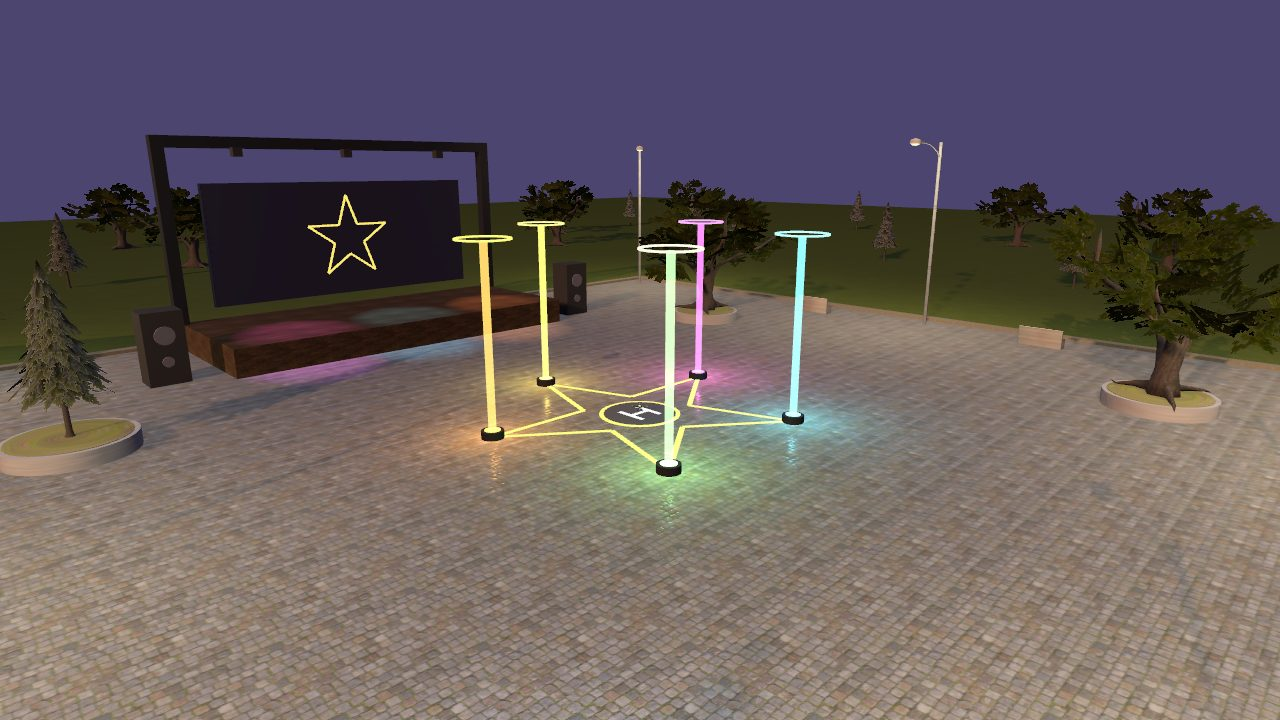
\includegraphics[width=\linewidth]{plaza_show_estrella}\\
    \credito{El mundo \cmd{plaza\_show} de \cmd{x500\_retos} (render propio)}
    \column{0.39\textwidth}\small
    Año nuevo en la plaza. El dron tiene que \textbf{dibujar una estrella en el cielo} pasando por los aros de
    luz.
    \begin{itemize}
      \item Mundo: \cmd{plaza\_show}.
      \item Nodo: \cmd{estrella\_show}, de \cmd{x500\_retos}.
      \item Viene de \cmd{square\_mission} (waypoints en offboard) y \cmd{orbit\_mission} (parámetros).
      \item \textbf{Lo nuevo}: los waypoints ya no se escriben a mano, se \textbf{calculan con una fórmula}.
    \end{itemize}
  \end{columns}
\end{frame}

\begin{frame}{Qué ya está hecho y qué te toca}
  \centering
  \begin{tikzpicture}[every node/.style={font=\scriptsize,align=center},
      es/.style={draw=verde,fill=verdeclaro,rounded corners,minimum width=1.75cm,minimum height=0.9cm}]
    \node[es] (w) at (0,0) {WARMUP};
    \node[es] (t) at (2.3,0) {TAKEOFF};
    \node[es] (s) at (4.6,0) {STAR};
    \node[es] (c) at (6.9,0) {CENTER};
    \node[es] (l) at (9.2,0) {LANDING};
    \node[es] (d) at (11.5,0) {DONE};
    \foreach \a/\b in {w/t,t/s,s/c,c/l,l/d} \draw[-{Stealth},thick] (\a) -- (\b);
    \node[draw=rojo,fill=red!8,rounded corners,line width=1pt,minimum width=3.2cm,minimum height=1cm] (v) at (4.6,-2.0)
      {\cmd{vertices()}\\\textbf{TODO 1 y 2}: \color{rojo}tu parte};
    \draw[-{Stealth},thick,rojo] (v) -- node[right,font=\tiny]{la lista de puntos} (s);
  \end{tikzpicture}
  \vspace{0.6em}

  \raggedright\small
  \begin{itemize}
    \item En \textcolor{verde}{verde}: ya funciona. Despega, recorre la lista, regresa al centro, aterriza y te
      dice qué tan bien lo hiciste.
    \item En \textcolor{rojo}{rojo}: \cmd{vertices()} regresa la lista de puntos de la estrella. Hoy regresa una
      lista \textbf{vacía}.
    \item Si lo corres sin hacer nada, despega, te avisa y aterriza:
  \end{itemize}
  \begin{terminal}{ros2 run x500\_retos estrella\_show}
vertices() regresó una lista vacía: falta el TODO. Aterrizando
  \end{terminal}
\end{frame}

\begin{frame}{La geometría, paso a paso}
  \begin{columns}[c]
    \column{0.47\textwidth}\centering
    \begin{tikzpicture}[scale=0.62]
      \draw[gray!20,step=1] (-5.6,-5.6) grid (5.6,5.6);
      \draw[-{Stealth},verde,thick] (0,-5.6) -- (0,5.9) node[above,font=\tiny] {N};
      \draw[-{Stealth},rojo,thick] (-5.6,0) -- (5.9,0) node[right,font=\tiny] {E};
      \draw[azul!50,thick] (0,0) circle (5);
      \draw[|-|,gris,visible on=<1>] (0,0) -- (-5,0) node[midway,below,font=\tiny] {R = radius};
      \draw[naranja!60,thick,visible on=<3->] (0,0) circle (1.91);
      % picos: ángulo 72k desde el norte hacia el este -> (E, N) = (R sen a, R cos a)
      \foreach \k in {0,...,4} {
        \pgfmathsetmacro{\a}{72*\k}
        \pgfmathtruncatemacro{\pp}{\k==0 ? 1 : 2}
        \pgfmathtruncatemacro{\ii}{\k==0 ? 3 : 4}
        \fill[azul,visible on=<\pp->] ({5*sin(\a)},{5*cos(\a)}) circle (4.5pt);
        \node[font=\tiny\bfseries,visible on=<\pp->] at ({5.7*sin(\a)},{5.7*cos(\a)}) {P\k};
        \pgfmathsetmacro{\b}{72*\k+36}
        \fill[naranja,visible on=<\ii->] ({1.91*sin(\b)},{1.91*cos(\b)}) circle (4pt);
        \node[font=\tiny\bfseries,visible on=<\ii->] at ({2.55*sin(\b)},{2.55*cos(\b)}) {I\k};
      }
      \draw[gris,visible on=<2>] (0,1.2) arc (90:18:1.2) node[midway,above right,font=\tiny] {72°};
      \draw[azul,line width=1.5pt,visible on=<5->,-{Stealth}]
        plot coordinates {(0,5) ({1.91*sin(36)},{1.91*cos(36)}) ({5*sin(72)},{5*cos(72)}) ({1.91*sin(108)},{1.91*cos(108)})
          ({5*sin(144)},{5*cos(144)}) ({1.91*sin(180)},{1.91*cos(180)}) ({5*sin(216)},{5*cos(216)})
          ({1.91*sin(252)},{1.91*cos(252)}) ({5*sin(288)},{5*cos(288)}) ({1.91*sin(324)},{1.91*cos(324)}) (0,5)};
      \only<5>{\node at (0,5) {\dronarriba{0.8cm}};}
    \end{tikzpicture}
    \column{0.5\textwidth}\small
    \only<1>{\textbf{1. El círculo.} Todos los picos están en un círculo de radio \cmd{radius} (5 m). El primero,
      \textbf{P0}, al norte.}%
    \only<2>{\textbf{2. Los picos.} Con \cmd{points} = 5 picos, entre uno y otro hay $360°/5 = 72°$. El pico
      $k$ está a un ángulo $\frac{2\pi k}{\text{points}}$ (en radianes) medido desde el norte hacia el este.
      \textbf{Esto es el TODO 1.}}%
    \only<3>{\textbf{3. El círculo de adentro.} Los vértices interiores están en un círculo más chico: radio
      \cmd{radius * inner\_ratio} ($5 \times 0.382 = 1.91$ m). \textbf{I0} va a la mitad, en ángulo, entre P0 y
      P1.}%
    \only<4>{\textbf{4. Todos los interiores.} Uno después de cada pico. \textbf{Esto es el TODO 2.} Si
      \cmd{inner\_ratio} es 0, no hay interiores.}%
    \only<5>{\textbf{5. El orden de vuelo.} P0, I0, P1, I1, \ldots, P4, I4 y de vuelta. Esa es la lista que
      \cmd{vertices()} tiene que regresar; el resto del nodo la vuela.}%
  \end{columns}
\end{frame}

\begin{frame}{De ángulo a norte y este}
  \begin{columns}[c]
    \column{0.42\textwidth}\centering
    \begin{tikzpicture}[scale=1.1]
      \draw[-{Stealth},verde,thick] (0,0) -- (0,2.7) node[above,font=\tiny] {Norte};
      \draw[-{Stealth},rojo,thick] (0,0) -- (2.7,0) node[right,font=\tiny] {Este};
      \draw[azul,thick] (0,0) -- (1.5,2.0);
      \fill[azul] (1.5,2.0) circle (2.5pt) node[above right,font=\tiny] {punto};
      \draw[dashed,gray] (1.5,2.0) -- (1.5,0) node[below,font=\tiny] {$r\sin a$};
      \draw[dashed,gray] (1.5,2.0) -- (0,2.0) node[left,font=\tiny] {$r\cos a$};
      \draw (0,0.7) arc (90:53:0.7); \node[font=\tiny] at (0.3,0.95) {$a$};
      \node[font=\tiny,azul] at (0.55,1.25) {$r$};
    \end{tikzpicture}
    \column{0.55\textwidth}\small
    Un punto a distancia $r$ y ángulo $a$ (desde el norte, girando hacia el este):
    \[ \text{norte} = r\cos a \qquad \text{este} = r\sin a \]
    En el código, cada vértice es \cmd{\{norte, este, z\}} con \cmd{z = -altitude} y se agrega con
    \cmd{out.push\_back(\{norte, este, z\});}
    \begin{ojo}
      \small
      \begin{itemize}
        \item \cmd{std::cos} y \cmd{std::sin} usan \textbf{radianes}, no grados.
        \item \cmd{k / points\_} con dos enteros da \textbf{0}: multiplica primero por \cmd{2 * M\_PI}.
        \item \cmd{radius\_} es \cmd{double} y el punto lleva \cmd{float}: \cmd{static\_cast<float>(...)}.
      \end{itemize}
    \end{ojo}
  \end{columns}
\end{frame}

\begin{frame}[fragile]{Pruébalo}
  \begin{lstlisting}[style=bash]
vespo up --sim --world plaza_show                     # terminal 1
ros2 run x500_retos estrella_show                     # terminal 2
# ... cambias vertices() en src/x500_retos/src/estrella_show.cpp ...
vespo build x500_retos                                # y otra vez ros2 run
  \end{lstlisting}
  \begin{columns}[c]
    \column{0.5\textwidth}
    \begin{terminal}{al final, si salió bien}
Aterrizado. Qué tan cerca pasó de cada vértice:\\
\ \ \ 1: 0.08 m OK\\
\ \ \ 2: 0.11 m OK\\
\ \ \ \ldots\\
\ \ 10: 0.09 m OK\\
Misión cumplida
    \end{terminal}
    \column{0.47\textwidth}\small
    \textbf{Se cumple si} pasa a menos de \textbf{0.5 m} de cada vértice, regresa al centro y aterriza. Si uno dice
    \textcolor{rojo}{FALLÓ}, ese punto quedó mal calculado.
  \end{columns}
\end{frame}

\begin{frame}[fragile]{Si tu fórmula es correcta, sirve para todo}
  \begin{columns}[t]
    \column{0.32\textwidth}\centering
    \begin{tikzpicture}[scale=0.32]
      \draw[azul,line width=1.2pt] plot coordinates {(0,5) ({1.91*sin(36)},{1.91*cos(36)}) ({5*sin(72)},{5*cos(72)}) ({1.91*sin(108)},{1.91*cos(108)})
          ({5*sin(144)},{5*cos(144)}) ({1.91*sin(180)},{1.91*cos(180)}) ({5*sin(216)},{5*cos(216)})
          ({1.91*sin(252)},{1.91*cos(252)}) ({5*sin(288)},{5*cos(288)}) ({1.91*sin(324)},{1.91*cos(324)}) (0,5)};
    \end{tikzpicture}\\
    \scriptsize por defecto\\\cmd{points:=5}
    \column{0.32\textwidth}\centering
    \begin{tikzpicture}[scale=0.32]
      \draw[azul,line width=1.2pt] plot coordinates {(0,5) ({2.5*sin(30)},{2.5*cos(30)}) ({5*sin(60)},{5*cos(60)}) ({2.5*sin(90)},{2.5*cos(90)})
          ({5*sin(120)},{5*cos(120)}) ({2.5*sin(150)},{2.5*cos(150)}) ({5*sin(180)},{5*cos(180)}) ({2.5*sin(210)},{2.5*cos(210)})
          ({5*sin(240)},{5*cos(240)}) ({2.5*sin(270)},{2.5*cos(270)}) ({5*sin(300)},{5*cos(300)}) ({2.5*sin(330)},{2.5*cos(330)}) (0,5)};
    \end{tikzpicture}\\
    \scriptsize\cmd{points:=6}\\\cmd{inner\_ratio:=0.5}
    \column{0.32\textwidth}\centering
    \begin{tikzpicture}[scale=0.32]
      \draw[azul,line width=1.2pt] (0,5) -- (5,0) -- (0,-5) -- (-5,0) -- cycle;
    \end{tikzpicture}\\
    \scriptsize\cmd{points:=4}\\\cmd{inner\_ratio:=0.0}: ¡un cuadrado!
  \end{columns}
  \vspace{0.4em}
  \begin{lstlisting}[style=bash]
ros2 run x500_retos estrella_show --ros-args -p points:=6 -p inner_ratio:=0.5
ros2 run x500_retos estrella_show --ros-args -p points:=4 -p inner_ratio:=0.0
  \end{lstlisting}
  \small Con 4 picos y sin interiores es el \cmd{square\_mission}, pero calculado: el mismo código hace las tres
  figuras.
\end{frame}

% =============================================================================
\section{Cuando algo no jala}
% =============================================================================

\begin{frame}{Revisa en este orden}
  \centering
  \begin{tikzpicture}[every node/.style={font=\scriptsize,align=center},
      q/.style={draw=azul,fill=azulclaro,rounded corners,text width=2.35cm,minimum height=1.25cm},
      f/.style={draw=rojo,fill=red!5,rounded corners,text width=2.35cm,minimum height=0.9cm,font=\tiny}]
    \node[q] (a) at (0,0) {\textbf{1} ¿\cmd{vespo doctor} sale todo en verde?};
    \node[q] (b) at (2.75,0) {\textbf{2} ¿Aparecen los topics \cmd{/fmu}?};
    \node[q] (c) at (5.5,0) {\textbf{3} ¿\cmd{telemetry\_listener} recibe datos?};
    \node[q] (d) at (8.25,0) {\textbf{4} ¿QGC dice \textbf{Ready To Fly}?};
    \node[q] (e) at (11,0) {\textbf{5} ¿En qué \textbf{modo} está? ¿Qué dice el monitor?};
    \foreach \x/\y in {a/b,b/c,c/d,d/e} \draw[-{Stealth},thick,verde] (\x) -- node[above,font=\tiny]{sí} (\y);
    \node[f] (fa) at (0,-1.9) {corre el \cmd{fix} que te dice};
    \node[f] (fb) at (2.75,-1.9) {¿corre el agente? \cmd{vespo down} y \cmd{vespo up -{}-sim}};
    \node[f] (fc) at (5.5,-1.9) {¿mismo \cmd{ROS\_DOMAIN\_ID}? ¿PX4 arrancó?};
    \node[f] (fd) at (8.25,-1.9) {lee el mensaje rojo de QGC; espera al GPS};
    \node[f] (fe) at (11,-1.9) {\cmd{flight\_mode\_monitor} dice qué hizo PX4};
    \foreach \x in {a,b,c,d,e} \draw[-{Stealth},thick,rojo] (\x) -- node[right,font=\tiny]{no} (f\x);
  \end{tikzpicture}
  \vspace{0.5em}

  \raggedright\small Casi siempre el problema está en el \textbf{primer} paso que falla. No te saltes pasos:
  revisar tu código cuando el agente ni siquiera corre es tiempo perdido.
\end{frame}

\begin{frame}{Síntoma, causa, arreglo (1/2)}
  \centering\scriptsize
  \begin{tabular}{p{4.1cm}p{4.3cm}p{4.6cm}}
    \toprule
    Ves & Casi siempre es & Haz \\
    \midrule
    \cmd{ros2 topic list} no tiene \cmd{/fmu} & el agente no corre & \cmd{vespo up -{}-sim} (o \cmd{vespo agent}) \\
    Tu nodo no recibe nada, sin error & nombre sin \cmd{\_v1}, o QoS \cmd{reliable} & copia nombre y QoS de un ejemplo \\
    \cmd{No executable found} & no compilaste, o paquete nuevo & \cmd{vespo build} y terminal nueva \\
    Cambiaste el código y hace lo mismo & no compilaste (o falló el build) & \cmd{vespo build}, lee los errores \\
    \cmd{UDP port 8888 busy} & quedó algo de antes & \cmd{vespo down} \\
    Gazebo lentísimo o la laptop se apaga & batería, o un proceso zombi & cargador; \cmd{vespo down} \\
    \bottomrule
  \end{tabular}
\end{frame}

\begin{frame}{Síntoma, causa, arreglo (2/2): el dron}
  \centering\scriptsize
  \begin{tabular}{p{4.1cm}p{4.3cm}p{4.6cm}}
    \toprule
    Ves & Casi siempre es & Haz \\
    \midrule
    No arma: ``No connection to the GCS'' & QGroundControl cerrado & ábrelo (\cmd{vespo qgc}); \cmd{vespo up} ya lo abre \\
    No arma recién arrancado & el GPS o el estimador aún no están listos & espera a \textbf{Ready To Fly} \\
    No entra a Offboard & no hubo setpoints antes & calienta 1 s antes de pedir el modo \\
    Sube y luego pasa a \textbf{Hold} & tu nodo dejó de publicar (Ctrl+C, crash, un \cmd{sleep}) & \cmd{flight\_mode\_monitor} lo confirma \\
    Se va a otro lado & confundiste NED: \cmd{z} positivo es \textbf{abajo}; x es norte & revisa signos y orden \\
    Llega y nunca pasa al siguiente WP & tolerancia muy chica o WP inalcanzable & imprime la distancia al WP \\
    Se desarma solo en tierra & armó y nadie le pidió despegar & normal: es seguridad de PX4 \\
    \bottomrule
  \end{tabular}
\end{frame}

\begin{frame}[fragile]{La hoja para tener a la mano}
  \begin{columns}[t]
    \column{0.5\textwidth}
    \begin{lstlisting}[style=bash,caption={vespo}]
vespo doctor          # todo bien?
vespo update          # lo nuevo del equipo
vespo build [PKG]     # compilar
vespo up --sim        # simulacion completa
vespo up --sim --world plaza_show
vespo down            # apagar todo
vespo simulate --show # modelos y mundos
vespo config          # mi configuracion
    \end{lstlisting}
    \column{0.47\textwidth}
    \begin{lstlisting}[style=bash,caption={ROS 2}]
ros2 run px4_examples telemetry_listener
ros2 run px4_examples flight_mode_monitor
ros2 topic list | grep fmu
ros2 topic echo /fmu/out/vehicle_status_v1 \
  --field nav_state
ros2 interface show px4_msgs/msg/<Tipo>
    \end{lstlisting}
    \scriptsize\textbf{nav\_state}: 4 Hold · 14 Offboard · 17 Takeoff · 18 Land · 5 Return
  \end{columns}
\end{frame}

\begin{frame}{Y después}
  \begin{columns}[c]
    \column{0.52\textwidth}\small
    \begin{enumerate}
      \item Corre los 18 ejemplos, con \cmd{flight\_mode\_monitor} al lado.
      \item Haz los ejercicios de \cmd{square\_mission}.
      \item Resuelve la \textbf{estrella}.
      \item Sigue con los retos de \cmd{x500\_retos}: el pilar, la entrega, la geocerca, la cueva\ldots
    \end{enumerate}
    \vspace{0.3em}
    \begin{idea}
      \small ¿Dudas de un mensaje o de un ejemplo línea por línea? Está todo en la \textbf{referencia técnica}
      (\cmd{referencia.pdf}).
    \end{idea}
    \column{0.45\textwidth}\centering
    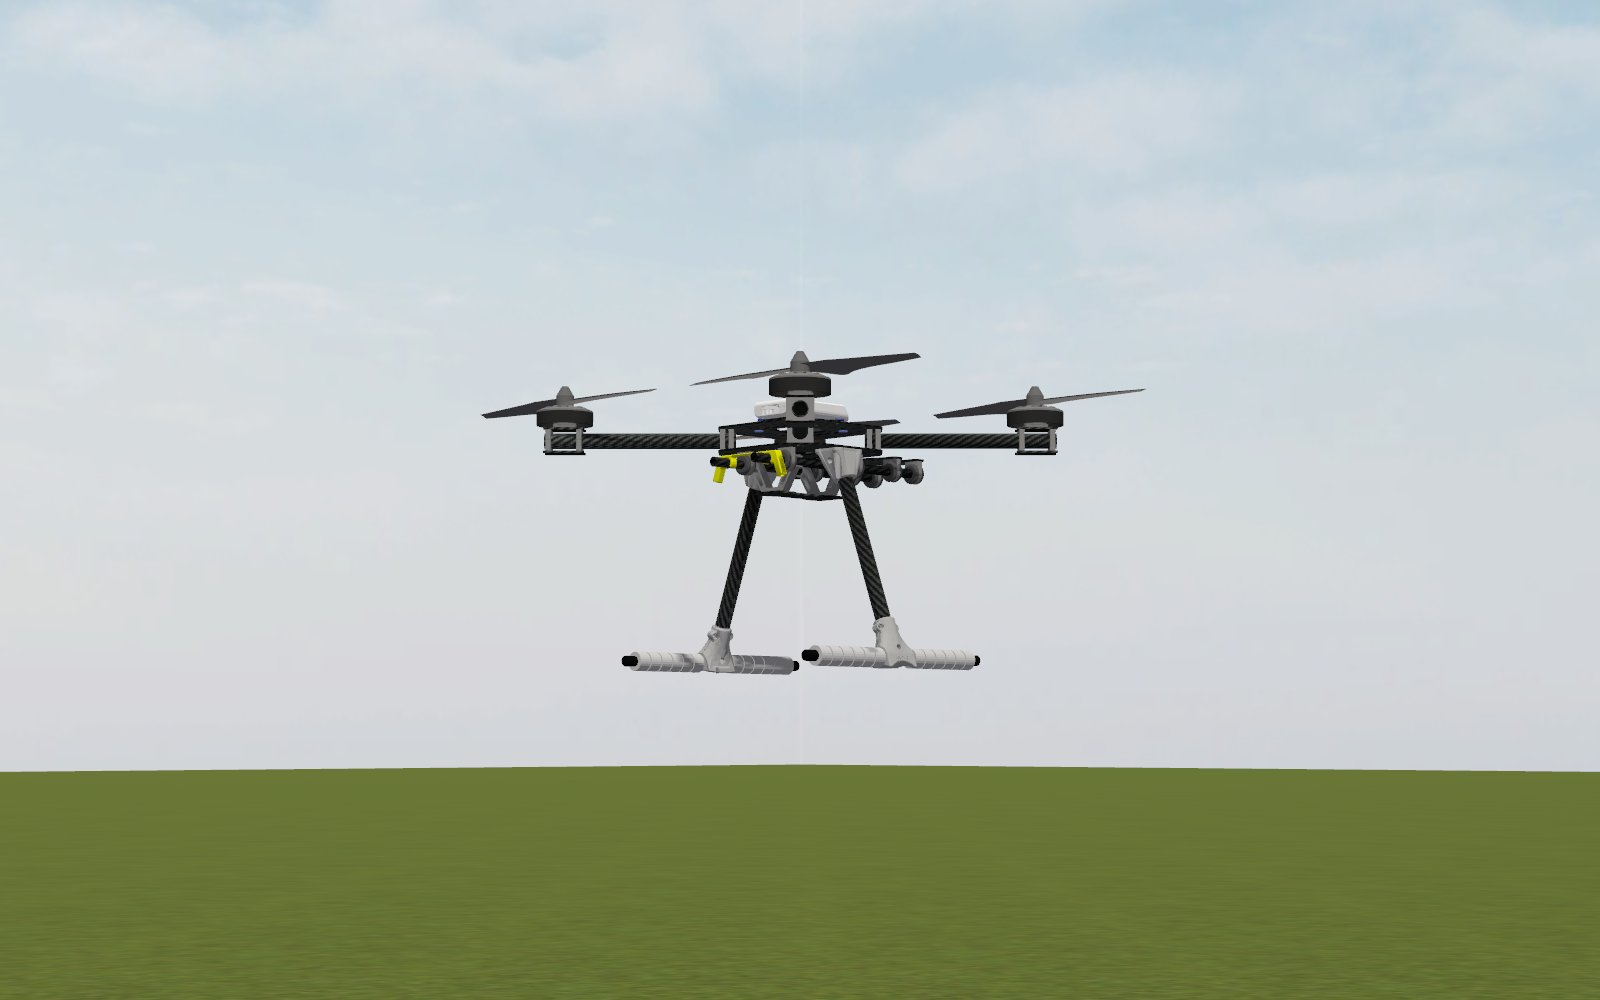
\includegraphics[width=\linewidth]{x500_volando}
  \end{columns}
\end{frame}


\begin{frame}{Créditos de las imágenes}
  \small
  \begin{itemize}
    \item \textbf{Capturas de QGroundControl y Gazebo, fotos y el diagrama de uXRCE-DDS}: documentación de PX4
      (\cmd{docs.px4.io}), © PX4 / Dronecode y colaboradores, licencia \textbf{CC BY 4.0}
      (\cmd{creativecommons.org/licenses/by/4.0}). Solo se redimensionaron.
    \item \textbf{Renders del x500 y de los mundos}: propios, con Gazebo Harmonic sobre el modelo \cmd{x500} de
      PX4 (\cmd{tools/renders\_x500.py}).
  \end{itemize}
  \vspace{0.6em}
  \centering
\includegraphics[height=1.4cm]{vespo_logo}
\end{frame}

\end{document}
